% UG project example file, February 2024
%
%   Added the "online" option for equal margins, February 2024 [Hiroshi Shimodaira, Iain Murray]
%   A minor change in citation, September 2023 [Hiroshi Shimodaira]
%
% Do not change the first two lines of code, except you may delete "logo," if causing problems.
\documentclass[logo,bsc,singlespacing,parskip,online]{infthesis}
\usepackage{ugcheck}

\usepackage{microtype} 
\usepackage[numbers,sort&compress]{natbib}
\usepackage{url}
\usepackage{graphicx}
\usepackage{booktabs}
\usepackage{float}
\usepackage{multirow}
\usepackage{array}
\usepackage{tabularx}
\usepackage[hidelinks]{hyperref}
\usepackage{xcolor}

\begin{document}
\begin{preliminary}

\title{Simulating Political Discourse on Twitter/X: An LLM-Integrated Agent-Based Model for Forward-Looking Thread Generation}
\author{Luke Tervit}
\course{Computer Science}
\project{4th Year Project Report}

\date{\today}

\abstract{
Most political social-media studies are retrospective: they explain observed engagement after publication but cannot run controlled, forward-looking tests of how a new post may shape reply dynamics. This dissertation addresses that gap with an LLM-integrated agent-based pipeline that generates synthetic political reply threads from only a root tweet and historically grounded agent profiles. Agent populations are constructed from classified USC~X~24 user histories (political leaning, emotion, sentiment, aggression), and Dolphin-Llama3~8B generates persona-conditioned replies over multi-round interaction. Across 100 held-out threads, the final pipeline achieves mean overall accuracy of $92.3\% \pm 4.6\%$ and composite fidelity of $0.857 \pm 0.106$, with no significant directional sentiment bias (Wilcoxon $p = 0.633$); political composition is the strongest-matching dimension (mean JSD $= 0.039$). A 21-configuration ablation and cross-model comparison (Dolphin-Llama3~8B vs Qwen2.5~7B) show that context window size, temperature, reply probability, and vocabulary conditioning drive most fidelity variation, while model choice primarily affects sentiment calibration. The main contribution is therefore a validated pipeline for thread-level counterfactual research, with the case study showing how the same instrument can support controlled message testing that engagement-only analysis and non-text ABMs cannot provide.
}

\maketitle

\newenvironment{ethics}
   {\begin{frontenv}{Research Ethics Approval}{\LARGE}}
   {\end{frontenv}\newpage}

\begin{ethics}
This project was planned in accordance with the Informatics Research
Ethics policy. It did not involve any aspects that required approval
from the Informatics Research Ethics committee.

\standarddeclaration
\end{ethics}

\begin{acknowledgements}
I thank my supervisor for guidance on methodology and evaluation design, and the School of Informatics for providing the computational infrastructure used to run large-scale experiments.
\end{acknowledgements}

\tableofcontents
\end{preliminary}

% ==========================================
% CHAPTER 1: INTRODUCTION
% ==========================================
\chapter{Introduction}

\section{Motivation}
Engagement metrics for political content on X (likes, reposts, reply counts) are easy to collect and useful for descriptive analysis, but they are weak proxies for latent reaction dynamics such as stance evolution, affective response, and hostility patterns~\citep{diehl2016political,bozdag2025survey}. This creates a practical gap: analysts can observe what content received attention, but cannot directly test how similar populations may react to a new tweet before deployment.

We address that gap with a forward-looking simulation pipeline. Given only a root tweet and a population of historically grounded agents, the system generates a synthetic reply thread and evaluates its realism against observed threads using distributional fidelity metrics~\citep{composta2025simulating,butler2024misinformation}. The aim is not to recover ``true'' internal psychological states, but to reproduce observable reaction patterns in language closely enough to support controlled research studies and bounded pre-deployment message analysis.

\section{Limitations of Current Approaches}
Current approaches often fall into two categories. First, predictive content models estimate engagement or label-level outcomes from historical features, but do not generate conversational trajectories. Second, classical opinion-dynamics ABMs such as bounded-confidence models represent agents with continuous or scalar opinions rather than generated language, making direct comparison with real social media discourse difficult~\citep{deffuant2000mixing,hegselmann2002opinion}.

As a result, there is limited work that can simultaneously (i) run in a strictly forward mode from a root tweet, (ii) generate realistic natural-language replies, and (iii) support quantitative validation against real thread-level distributions across sentiment, politics, emotion, and aggression.

\section{Core Thesis Claim}
The core claim of this dissertation is that an LLM-integrated ABM can function as a \emph{new research instrument} for political communication: not just describing past platform behaviour, but enabling controlled forward simulations of likely reply dynamics for unseen posts. This shifts the methodological unit of analysis from retrospective engagement correlation to prospective thread generation under explicit behavioural assumptions.

Concretely, the pipeline enables study designs that are difficult or impossible with prior methods: (i) counterfactual root-tweet edits while holding audience composition fixed, (ii) ex-ante estimation of downstream sentiment, stance, emotion, and aggression trajectories, and (iii) stress-testing claims from observational papers in a controlled simulated environment. The same capability also has practical value for message design workflows, where the goal is to compare likely discourse effects of alternative phrasings before publication under clearly stated modelling assumptions.

\section{Project Objectives}
This dissertation has four objectives:
\begin{enumerate}
\item Build an LLM-integrated ABM that simulates reply-thread dynamics from a root tweet without using target-thread reply data.
\item Construct agent populations from historical user profiles so that simulation participants reflect empirical behavioural heterogeneity.
\item Evaluate simulation realism at scale on 100 held-out political threads using multi-metric fidelity analysis and statistical testing.
\item Compare model choices and behavioural design decisions through ablation and cross-model experiments.
\end{enumerate}

\section{Contributions}
This dissertation makes four main contributions.
\begin{itemize}
\item \textbf{A novel forward-simulation pipeline}: a text-generating ABM+LLM system that predicts full reply-thread trajectories from a root tweet, enabling counterfactual studies and bounded message-testing workflows that engagement-only analytics and non-text ABMs cannot run.
\item \textbf{An empirically grounded agent construction workflow}: agent behavioural profiles are derived from historical tweet data, producing simulation populations that preserve observed political and linguistic heterogeneity.
\item \textbf{A reproducible thread-level validation protocol}: 100-thread evaluation with per-thread metrics across sentiment, political stance, emotion, aggression, and volume, supporting direct comparison between synthetic and real discourse.
\item \textbf{Evidence of what makes the pipeline useful}: a 21-configuration ablation study, cross-model comparison (Dolphin-Llama3 8B vs Qwen2.5 7B), and counterfactual case study that isolate the design choices and use cases most responsible for its value.
\end{itemize}

% ==========================================
% CHAPTER 2: BACKGROUND AND RELEVANT WORK
% ==========================================
\chapter{Background and Relevant Work}

\section{Problem Framing: Engagement vs Reaction Dynamics}
Prior work has identified emotional tone, framing, and source cues as important correlates of political message spread, but most analyses remain retrospective and engagement-centric~\citep{bozdag2025survey,diehl2016political,antypas2023negativity,geels2024virtuallabcoats,dumas2022influencers}. These approaches explain what happened after publication, but they do not provide a controlled way to test likely downstream reply dynamics for unseen content.

This gap motivates simulation-oriented approaches that estimate observable reaction trajectories rather than latent ``true'' psychology~\citep{butler2024misinformation,composta2025simulating}. In this dissertation, reaction quality is operationalised through measurable thread-level outcomes: sentiment and political distributions, emotion mix, aggression level, and reply volume. That framing matters because the pipeline is designed to answer ``what happens next if the post changes?'' rather than ``what features correlated with engagement last time?''

This chapter reviews existing research on LLM-based social simulation, online political discourse dynamics, and measurement limitations of engagement-only evaluation.

\section{Previous Work}

The simulation of social dynamics has a long history in agent-based modelling. Classical opinion dynamics models such as the bounded confidence model~\citep{deffuant2000mixing} and the Hegselmann--Krause model~\citep{hegselmann2002opinion} represent agents as scalar opinion values updated through pairwise interaction rules: agents influence one another when their opinions fall within a threshold distance, producing convergence clusters and polarisation as emergent outcomes. These models established the theoretical foundations for understanding opinion formation and partisan entrenchment, but they do not produce text, making their outputs incomparable to real social media data.

More recently, large language models have been used to create agents capable of generating natural-language behaviour. Park et al.~\citep{park2023generative} demonstrated that LLM-driven agents with detailed behavioural profiles can simulate believable human-like interactions in an open-ended sandbox environment, establishing that persona-conditioned generation is a viable approach to social simulation. In the political domain, Composta et al.~\citep{composta2025simulating} calibrated LLM agents on real-world conversations from the 2022 Italian election and implemented a simulator with activity patterns fitted on Bluesky data, finding that AI agents were able to generate content, build social network structure, and align with real in-group interaction patterns to a median correlation of 0.85.

The key difference in our pipeline is how those personas are constructed. Rather than assigning agent characteristics through researcher-written prompt descriptions alone, we derive each agent profile from historical user tweets classified by five Twitter-specialised models. That gives the simulator a firmer empirical basis for political leaning, emotion, sentiment, and aggression before any generation step occurs.

These studies show that profile-conditioned generation is plausible, but they stop short of the main goal of this dissertation. Many LLM simulation papers evaluate aggregate interaction structure rather than full thread-level text generation and fidelity assessment, while many political-language systems focus on pairwise judgement or moderation tasks rather than end-to-end reply-thread simulation~\citep{ji2018coattention,mohammadi2025aifeedback}. We therefore build on that literature in a more specific direction: strict forward generation from a root tweet, full-thread text output, and thread-level quantitative validation.

\section{Reaction Mechanisms in Online Political Discourse}
Online political discourse often exhibits reinforcement and conversion-like patterns: users may become more entrenched in prior views or shift toward new framings depending on context, identity, and interaction structure~\citep{druckman2022framework,diehl2016political}. On platforms such as X, these processes play out through rapid public reply chains where language, affect, and visibility co-evolve over time.

This matters for the simulator because agent replies should depend on both stable persona tendencies and the local conversational state. That is why the pipeline combines history-informed agent profiles with round-based interaction and rolling thread context, rather than treating each reply as an isolated text-generation task.

\section{Measurement Challenges in Social Media Studies}
Research identifies several factors that shape large-scale reaction patterns on platforms such as X, including content structure, emotional tone, language style, and social proof mechanisms~\citep{brady2017emotion,geels2024virtuallabcoats,dumas2022influencers}.

Existing social media studies of political communication typically proxy downstream reaction with engagement metrics (likes, shares, comments), assuming that behavioural engagement indicates latent attitudinal response~\citep{diehl2016political}.

That assumption is too weak for the questions pursued here. If the goal is to compare alternative phrasings, test diffusion claims, or anticipate downstream tone before publication, the evaluation target has to be the reply thread itself. This is why the dissertation validates sentiment, politics, emotion, aggression, and volume directly instead of relying on engagement as a stand-in.

\section{Positioning of This Work}
The dissertation sits between descriptive social-media analytics and purely theoretical opinion-dynamics models. It uses LLM-based ABM to generate thread text, then validates the result against real threads with explicit quantitative metrics. The aim is predictive simulation of observable reaction dynamics under clear modelling assumptions, rather than direct inference of internal psychological truth. In practical terms, the contribution is a validated pipeline for prospective and counterfactual thread-level experimentation, with the later case study showing one of the most useful designs that this pipeline enables.

Table~\ref{tab:approach_feature_compare} makes that positioning concrete. The main distinction is not only that this system generates text, but that it combines forward generation with history-grounded agent construction and thread-level quantitative validation.

\begin{table}[ht]
\centering
\caption{Feature comparison between common approach classes and this dissertation.}
\label{tab:approach_feature_compare}
\small
\setlength{\tabcolsep}{5pt}
\renewcommand{\arraystretch}{1.15}
\begin{tabularx}{\textwidth}{@{}>{\raggedright\arraybackslash}p{0.24\textwidth}>{\raggedright\arraybackslash}X>{\centering\arraybackslash}p{0.14\textwidth}>{\centering\arraybackslash}p{0.13\textwidth}>{\raggedright\arraybackslash}p{0.21\textwidth}@{}}
\toprule
\textbf{Approach} & \textbf{Persona Basis} & \textbf{Root-Only Forward?} & \textbf{Full Thread Text?} & \textbf{Thread-Level Validation?} \\
\midrule
Engagement prediction models & Aggregate historical features & No & No & Usually limited \\
Classical opinion-dynamics ABMs & Assumed scalar opinion states & Yes & No & Not directly text-comparable \\
LLM agent demos with prompt-defined personas & Researcher-written prompts or manually assigned profiles & Sometimes & Sometimes & Varies \\
\textbf{This dissertation} & \textbf{Five-model historical user profiles} & \textbf{Yes (0-shot)} & \textbf{Yes} & \textbf{Yes (100 threads)} \\
\bottomrule
\end{tabularx}
\end{table}

% ==========================================
% CHAPTER 3: METHODOLOGY
% ==========================================
\chapter{Methodology}

\section{Research Design}

We adopt an agent-based modelling (ABM) approach because political reply threads are emergent systems: the thread-level sentiment, political mix, and reply volume that observers see are the aggregate result of many individual users deciding whether to reply, who to reply to, and what to say~\citep{diehl2016political,smith2021twitterbehaviors,smith2022politicalcontent}. ABM is therefore the right starting point. Instead of modelling the aggregate distribution directly, it models local interactions and lets thread-level outcomes emerge from them~\citep{axelrod1997complexity,epstein1996growing}.

The key methodological move is to integrate large language model (LLM) generation into the ABM agent loop. Classical opinion-dynamics ABMs represent agents as scalar opinion values updated by mathematical rules~\citep{deffuant2000mixing,hegselmann2002opinion}; that gives analytical simplicity, but no text output and therefore no direct comparison with real social-media threads. By contrast, an LLM-conditioned ABM produces observable language that can be analysed with the same tools used on real threads~\citep{butler2024misinformation,composta2025simulating}. The trade-off is greater modelling complexity, but that complexity is what makes thread-level validation possible.

The research question is predictive: given only the content of a root tweet, can the system generate a realistic simulation of the thread that forms around it? That requirement forces a fully forward design: no real reply data from the target thread may be used as input. The pipeline must generalise from historical user behaviour to unseen posts, which is why evaluation matters as much as generation quality.

\section{Theoretical Framework}

\subsection{Bounded Confidence}

The bounded confidence model~\citep{deffuant2000mixing} provides the theoretical basis for agent interaction selection. Under bounded confidence, an agent will only update its opinion in response to messages from agents whose position falls within a threshold distance of its own. Messages from agents outside this threshold are ignored. In the context of this simulation, bounded confidence governs which posts an agent is likely to engage with: agents are more likely to target posts from agents with similar or moderately opposing political orientations, and less likely to engage with posts from agents at the ideological extreme relative to their own position~\citep{diehl2016political,composta2025simulating}. The bounded confidence threshold is a free parameter of the model (set at 0.3 on a [0, 1] political distance scale in the present implementation) and is a subject of sensitivity analysis.

\subsection{The Backfire Effect}

The backfire effect~\citep{nyhan2010corrections} describes the empirical observation that exposure to information directly contradicting a strongly held belief can, in some individuals, entrench that belief rather than revise it. In the ABM, this is operationalised as a reply-targeting rule: agents with high aggression scores (hate\_score + offensive\_score $>$ 0.7) who encounter posts at extreme ideological distance ($>$ 0.6 on the political scale) are more likely to produce hostile, confrontational replies than to update toward the opposing view~\citep{druckman2022framework,diehl2016political,brady2017emotion}. This produces the partisan entrenchment and cross-ideological attack patterns that are characteristic of real political threads.

\subsection{Agent DNA as Behavioural Profile}

Each active agent is characterised by a DNA profile derived from their historical Twitter activity: political leaning (Left / Centre / Right), political confidence score, dominant emotion, sentiment orientation, hate speech likelihood, and offensive language likelihood. These dimensions were selected because they capture the key axes along which political Twitter users differ in their likely behaviour~\citep{antypas2023negativity,tun2023sentiment,smith2022politicalcontent}. The hate and offensive scores are combined into a single aggression parameter that governs reply probability, tone tier selection, and backfire effect activation. Political leaning and its associated confidence score govern target selection and opinion distance calculation.

\section{Data Source}

\subsection{USC X 24 Dataset}

The primary data source is the USC X 24 dataset, a large-scale collection of Twitter/X posts gathered during the 2024 US presidential election period. The full published dataset contains over forty million tweets collected via the Twitter/X API under academic research access. We use the May--July 2024 subset, comprising approximately 2.3 million tweets with reply chains, view counts, and user metadata. This period provides dense, politically salient interaction and frequent cross-partisan exchange, making it suitable for both agent construction and held-out thread evaluation.

\subsection{Thread Selection}

Threads were selected for simulation using two criteria. First, each thread needed enough replies to support meaningful ground-truth comparison; we required at least ten observed replies. Second, each thread needed some cross-partisan engagement, because ideologically homogeneous threads provide little leverage for testing bounded confidence and backfire-style mechanisms~\citep{diehl2016political,composta2025simulating,cetinkaya2025crosspartisan}. During development, we used a January 6th Capitol-attack thread as the main diagnostic case because it satisfied both criteria and made distributional errors easy to inspect.

For large-scale validation and ablation, we then drew 100 threads spanning varied topics, political compositions, and thread sizes. That broader sample tests whether the pipeline works beyond one illustrative thread and turns the dissertation from a case demo into an instrument evaluation.

\subsection{Agent Population Construction}

For each selected thread, the active agent population was constructed by matching the user IDs of thread participants against the classified agent DNA profiles derived from the full dataset. This produced a set of agents with empirically grounded behavioural profiles rather than synthetic, assumed ones. The political distribution, emotional register, and aggression levels of the agent population therefore reflected the actual users who participated in each thread --- a key distinction from prior work that typically initialises agents with theoretically assumed distributions (e.g., uniform or normal opinion distributions)~\citep{composta2025simulating}. It also differs from prompt-only persona assignment: the prompt does not invent the persona from scratch, but translates a profile already estimated from historical behaviour.

\section{Simulation Design}

\subsection{Simultaneous Activation}

The simulation used a simultaneous (synchronous) activation schedule: in each round, agents are evaluated against the same current thread state, and only those that pass the reply-probability step generate pending replies. Those pending replies are then committed simultaneously. This prevents sequential activation bias, in which agents that act earlier in a round would see a different thread state from those that act later, introducing an ordering artefact. Simultaneous activation therefore ensures that all responding agents act on the same conversational snapshot, consistent with the near-simultaneous nature of real social media engagement~\citep{butler2024misinformation}.

\subsection{Reply Probability and Target Selection}

An agent's probability of generating a reply in a given round was set as a base probability (5\%) modified by a linear function of the agent's aggression score, capped at a maximum. This reflects the empirical observation that more hostile and emotionally activated users are more likely to engage in online political discourse~\citep{antypas2023negativity,brady2017emotion}. Target selection weighted recent posts more heavily than older posts, and weighted ideologically proximate or moderately opposing posts according to the bounded confidence and backfire rules. The controversy weight parameter controlled the strength of the cross-partisan targeting tendency~\citep{cetinkaya2025crosspartisan}.

\subsection{Text Generation}

Each agent's reply was generated by Dolphin-Llama3 8B conditioned on a system prompt constructed from that agent's DNA profile. The system prompt described the agent's political orientation in terms of values and attitudes rather than categorical labels, included banks of politically charged vocabulary matched to the agent's ideology, assigned an aggression-appropriate tone tier scaled relative to the thread's mean aggression, and included an explicit set of behavioural rules preventing the model from identifying itself as an AI or echoing its own prompt structure. The user prompt was run in 0-shot mode and contained two components: the eight most recent posts in the simulated thread as conversational context, and the specific post being replied to. No real reply text from the target thread was injected into generation prompts.

\subsection{Core Simulation Procedure (Pseudocode)}

Table~\ref{tab:sim_loop_pseudocode} summarises the core synchronous simulation loop implemented in this dissertation.

\begin{table}[ht]
\centering
\caption{Core synchronous ABM simulation loop (simplified pseudocode).}
\label{tab:sim_loop_pseudocode}
\small
\begin{tabular}{p{0.06\textwidth}p{0.88\textwidth}}
\toprule
\textbf{Ln} & \textbf{Procedure} \\
\midrule
1  & \texttt{Input: root\_tweet, agents\_for\_thread, config (max\_rounds, behaviour params)} \\
2  & Initialise \texttt{thread\_history} with root tweet; initialise model state and counters \\
3  & \texttt{for t = 1 to max\_rounds:} \\
4  & \hspace{4mm}\texttt{pending\_replies = [ ]} \\
5  & \hspace{4mm}\texttt{for each agent a in active\_agents:} \\
6  & \hspace{8mm}Compute reply probability from base rate + aggression scaling \\
7  & \hspace{8mm}If sampled to reply: select target post using confidence/backfire rules \\
8  & \hspace{8mm}Build persona-conditioned prompt from DNA + recent thread context \\
9  & \hspace{8mm}Generate reply with Dolphin-Llama3; append to \texttt{pending\_replies} \\
10 & \hspace{4mm}Commit all \texttt{pending\_replies} simultaneously to \texttt{thread\_history} \\
11 & \hspace{4mm}Update per-round metrics (volume, aggression, stance/emotion summaries) \\
12 & \hspace{4mm}\texttt{if} stopping condition met (no activity or round cap): \texttt{break} \\
13 & Export simulation artefacts (\texttt{thread\_history.json}, \texttt{simulated\_thread\_metadata.json}, timeseries) \\
\bottomrule
\end{tabular}
\end{table}

\section{Validation Methodology}

\subsection{Classification of Generated Text}

All generated tweets were classified through the same five RoBERTa models used to construct the original agent DNA profiles: political leaning, emotion, sentiment, hate speech, and offensive language. This keeps the measurement pipeline consistent between real and simulated data, reducing the risk that apparent agreement or disagreement is caused by changing evaluators rather than changing text~\citep{antypas2023negativity,tun2023sentiment}. The trade-off is that classifier bias affects both construction and evaluation, which we treat later as a validity threat rather than hiding it.

\subsection{Distribution Comparison via Jensen--Shannon Divergence}

For each categorical dimension (political leaning, emotion, sentiment), the distribution of labels across all tweets in the thread was computed for both the real and simulated threads. Jensen--Shannon Divergence (JSD) was then computed between these distributions. JSD was selected over alternatives such as the $\chi^2$ statistic or mean absolute error because it is symmetric ($\text{JSD}(P\|Q) = \text{JSD}(Q\|P)$), bounded on $[0, 1]$, and well-defined when either distribution assigns zero probability to a category --- a common occurrence in short threads where some sentiment categories may be entirely absent. In this study, JSD values below 0.15 were treated as indicating good similarity between real and simulated distributions.

\subsection{Continuous Sentiment Score and Bias Testing}

In addition to the categorical sentiment label, a continuous sentiment score was derived from the raw model probability outputs: $P(\text{positive}) - P(\text{negative})$, yielding a value on $[-1, +1]$. This continuous score enabled per-thread paired comparison between real and simulated mean sentiment, and the computation of the sentiment residual (simulated mean $-$ real mean) as an indicator of directional bias.

To test for systematic bias across the full set of threads, a Wilcoxon signed-rank test was applied to the per-thread sentiment residuals. The Wilcoxon test was selected over the paired $t$-test because it makes no assumption of normality in the distribution of residuals, which cannot be guaranteed given the diversity of thread types and sizes. A statistically significant result ($p < 0.05$) indicates that the simulation exhibits a consistent directional bias across threads; a non-significant result indicates that observed differences are consistent with random variation.

\subsection{Weighted Overall Accuracy}

An overall accuracy score was computed as a weighted combination of the three JSD-based similarity scores and the normalised aggression gap:

\begin{equation}
\begin{array}{l}
\text{Overall} = 0.30 \times (1 - \text{Political JSD}) + 0.20 \times (1 - \text{Emotion JSD}) \\
\qquad\quad + 0.30 \times (1 - \text{Sentiment JSD}) + 0.20 \times (1 - \text{normalised aggression gap})
\end{array}
\end{equation}

Sentiment and political alignment were weighted equally as the primary behavioural dimensions; emotion and aggression calibration were weighted equally as secondary dimensions. Threads were rated EXCELLENT ($\geq 80\%$), GOOD (60--79\%), FAIR (40--59\%), or POOR ($< 40\%$).

\section{Experimental Design}

\subsection{Pipeline Validation (100 Threads)}

The first experiment asks a simple question: does the redesigned pipeline work at all beyond the development thread? We answer that with a 100-thread batch run. This is not a tuning exercise; parameters are held constant so the result reflects pipeline viability, not search over settings.

\subsection{Parameter Optimisation}

The second experiment asks whether the most serious failure mode can be repaired without breaking the rest of the system. After identifying systematic negative sentiment bias in the initial pipeline (mean residual $-0.390$, Wilcoxon $p = 4.27 \times 10^{-18}$), we implement the coordinated prompt changes described in Chapter~4 and re-run validation on the same 100-thread corpus to measure the reduction in bias and the effect on overall fidelity.

\subsection{Ablation Study}

The third experiment asks which design choices actually matter. To answer that, we run a 21-configuration ablation study. Each configuration is either a single-parameter departure from the optimised baseline --- varying temperature, context window size, aggression tier design, reply probability, controversy weight, vocabulary injection, repeat penalty, response length, and simulation length --- or one of five multi-parameter combinations. Each configuration is evaluated across 10 threads, yielding 210 total simulations. We rank configurations with a composite score combining sentiment JSD, temporal decay, lexical diversity (TTR), semantic drift, emotion trajectory, Gini coefficient, Spearman rank correlation, and stance consistency.

This follows standard controlled ablation logic from NLP and machine learning, adapted to an ABM setting where ``performance'' is not a single loss value but similarity to observed discourse along several dimensions.

\section{Ethical Considerations}

All tweet data used in this study was collected under academic research access to the Twitter/X API and forms part of the publicly available USC X 24 dataset. No personally identifiable information beyond user IDs (which are public) was used in the analysis. Agent DNA profiles aggregate behaviour across many tweets rather than representing individual posts, further reducing the risk of identifying specific users from model outputs. The simulation generates entirely synthetic text; no generated content is attributed to real individuals. The use of an uncensored language model to generate realistic hostile political language was judged necessary for scientific validity --- a model that cannot reproduce the hostility of real discourse cannot serve as a valid simulation instrument --- and all generated content remained within the closed research environment.

% ==========================================
% CHAPTER 4: IMPLEMENTATION
% ==========================================
\chapter{Implementation}

\section{Overview}

Implementation proceeded as a sequence of failures, diagnoses, and redesigns rather than as a one-pass build. That matters methodologically: the final pipeline did not emerge from prompt tweaking alone, but from repeated comparison against real-thread behaviour. The end result has three components: an agent-classification stage that derives behavioural profiles from historical tweets, a discourse-simulation stage that generates synthetic thread activity, and a validation stage that compares simulated output with real data. The sections that follow explain how each component changed, why it changed, and what evidence justified the redesign.

\section{Implementation Pipeline Diagrams}

Figure~\ref{fig:personality_extraction_pipeline} shows how historical tweet data is converted into agent DNA. The sequence matters: raw tweet chunks are cleaned, classified by the five-model bank, converted into tweet-level records, and then aggregated into one user-level profile. That is the core reason the personas are empirically grounded rather than written directly into the prompt.

\begin{figure}[H]
\centering
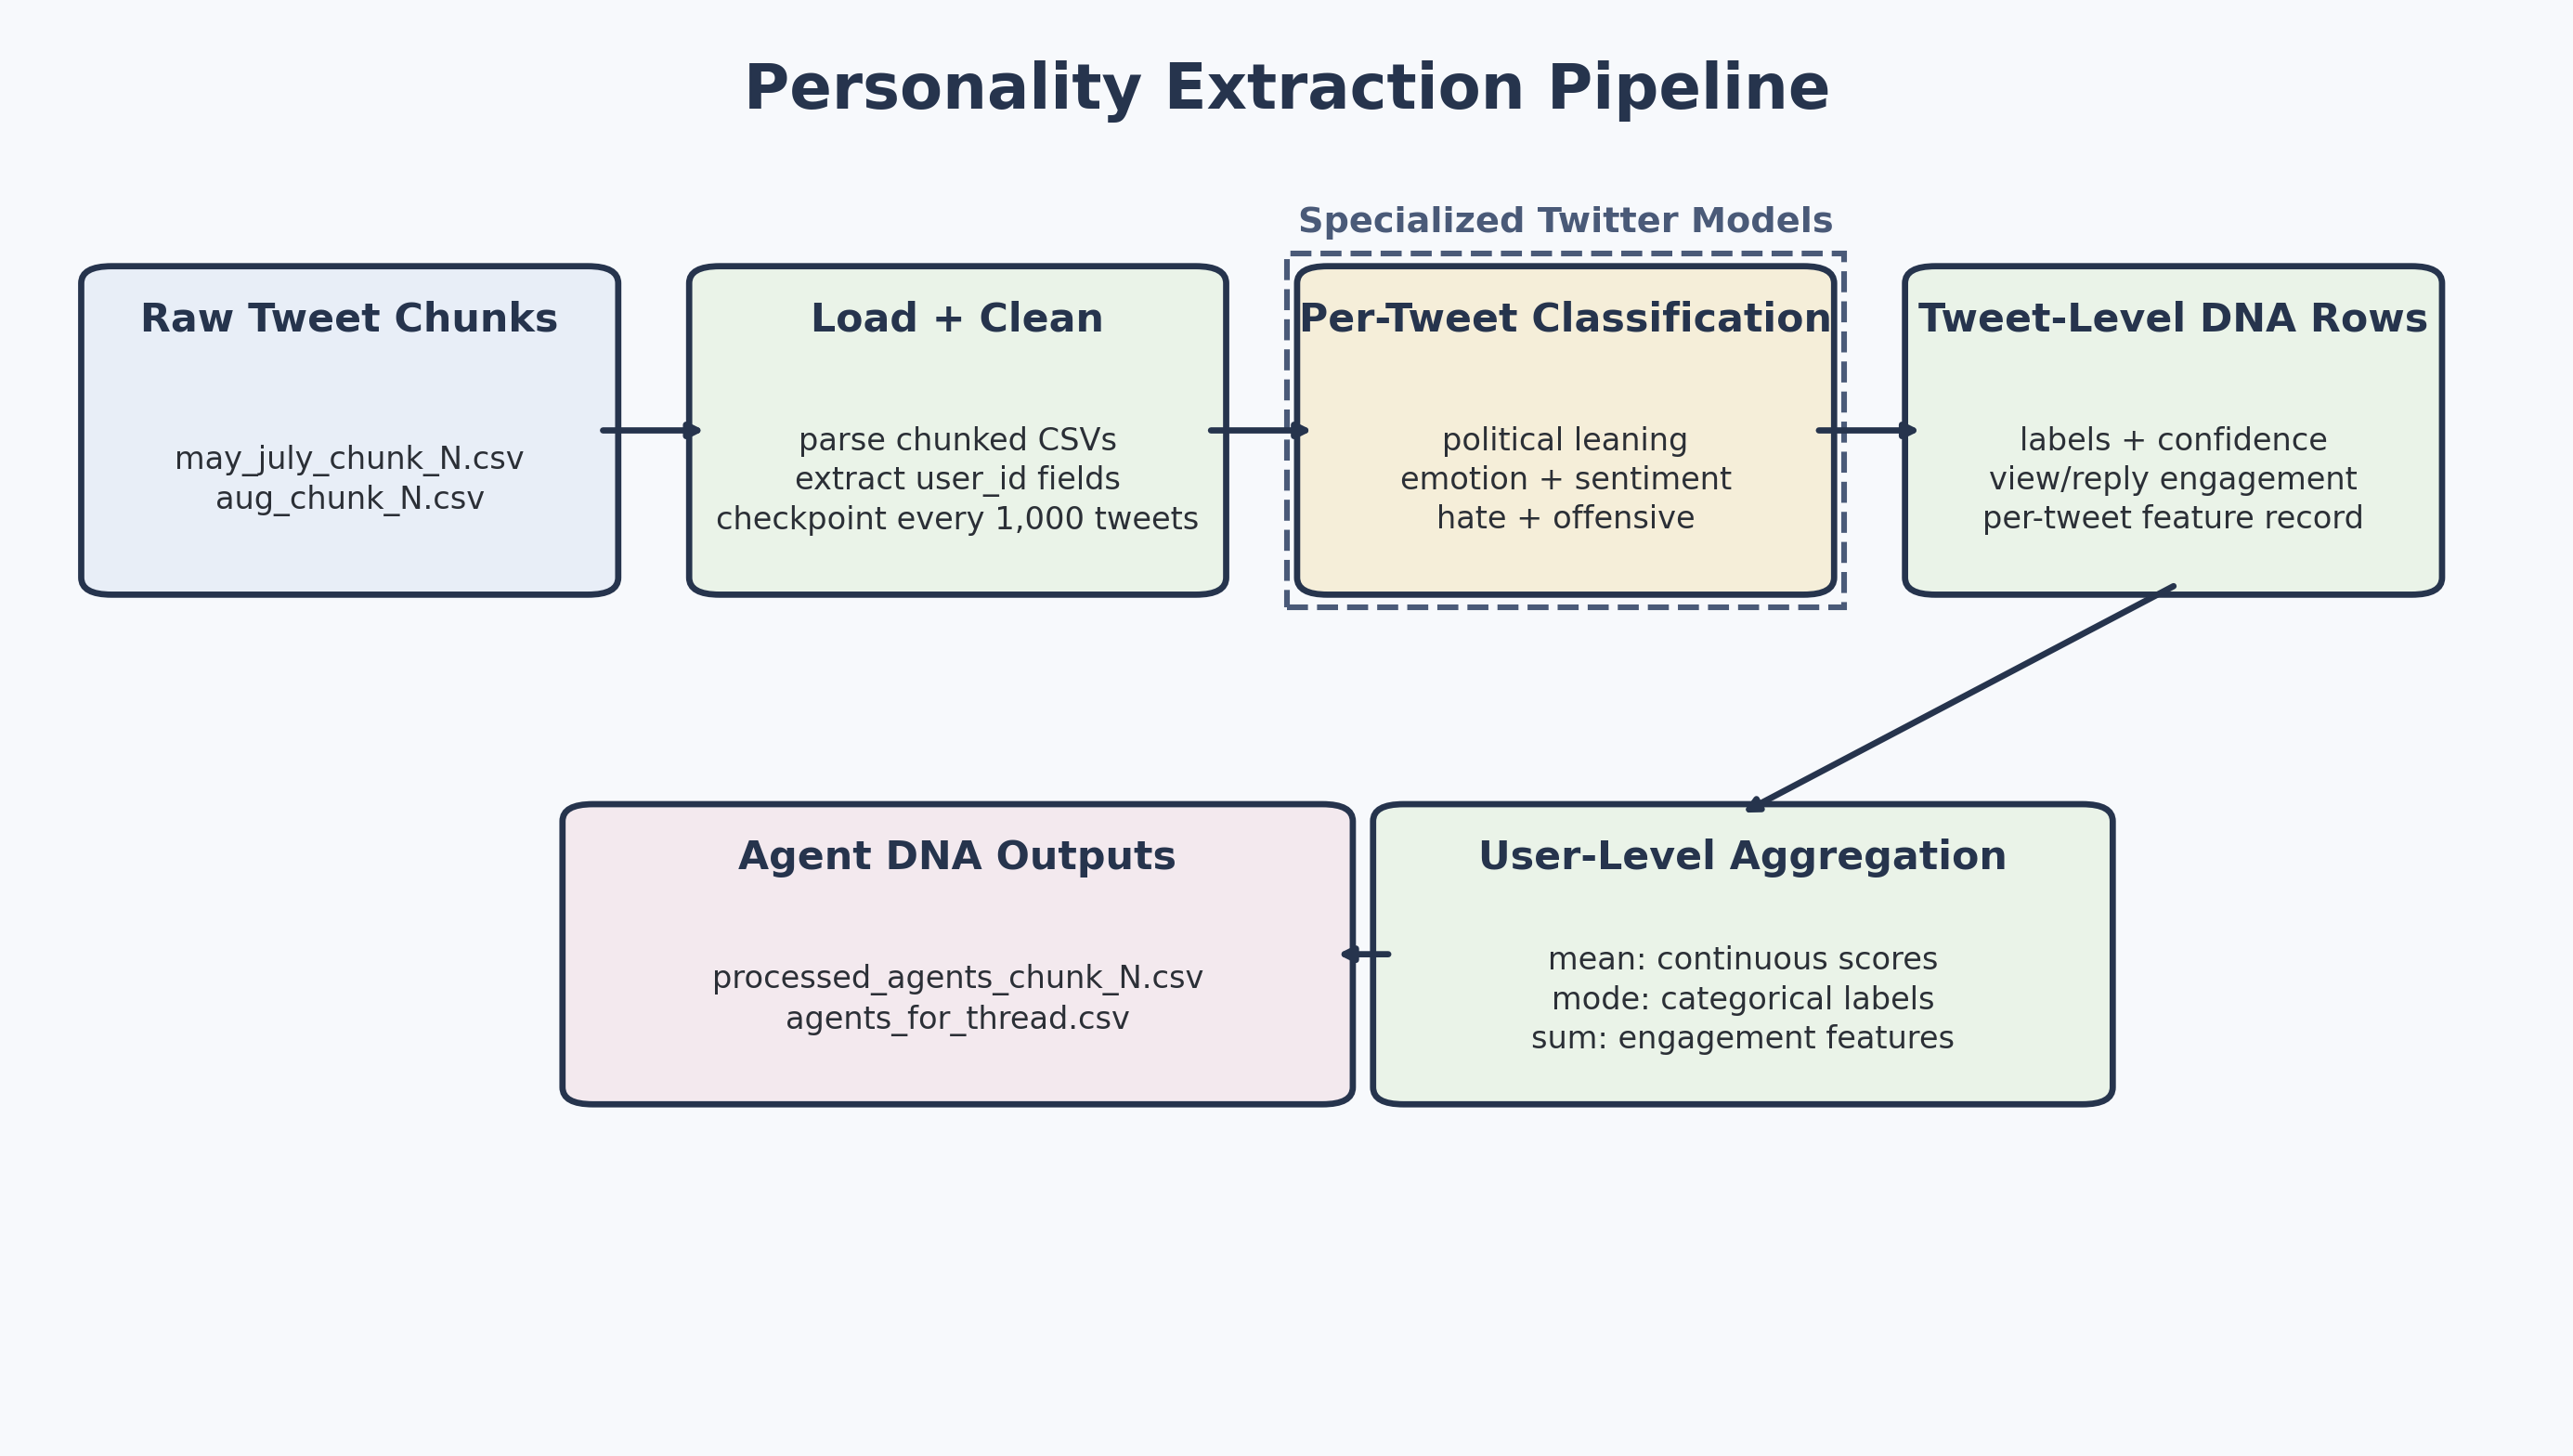
\includegraphics[width=\textwidth]{dissertation_figures/final/01_personality_extraction_pipeline.png}
\caption{Personality extraction pipeline used in the final system. Historical tweets are cleaned, classified by five specialised Twitter models, and aggregated into one behavioural profile per user.}
\label{fig:personality_extraction_pipeline}
\end{figure}

Figure~\ref{fig:simulation_pipeline} shows the forward simulation loop itself. The important point is the separation between the generate stage and the commit stage: reply decisions and pending generations are formed against a shared thread state, then committed synchronously. That structure keeps the simulation forward-looking while avoiding sequential activation artefacts.

\begin{figure}[H]
\centering
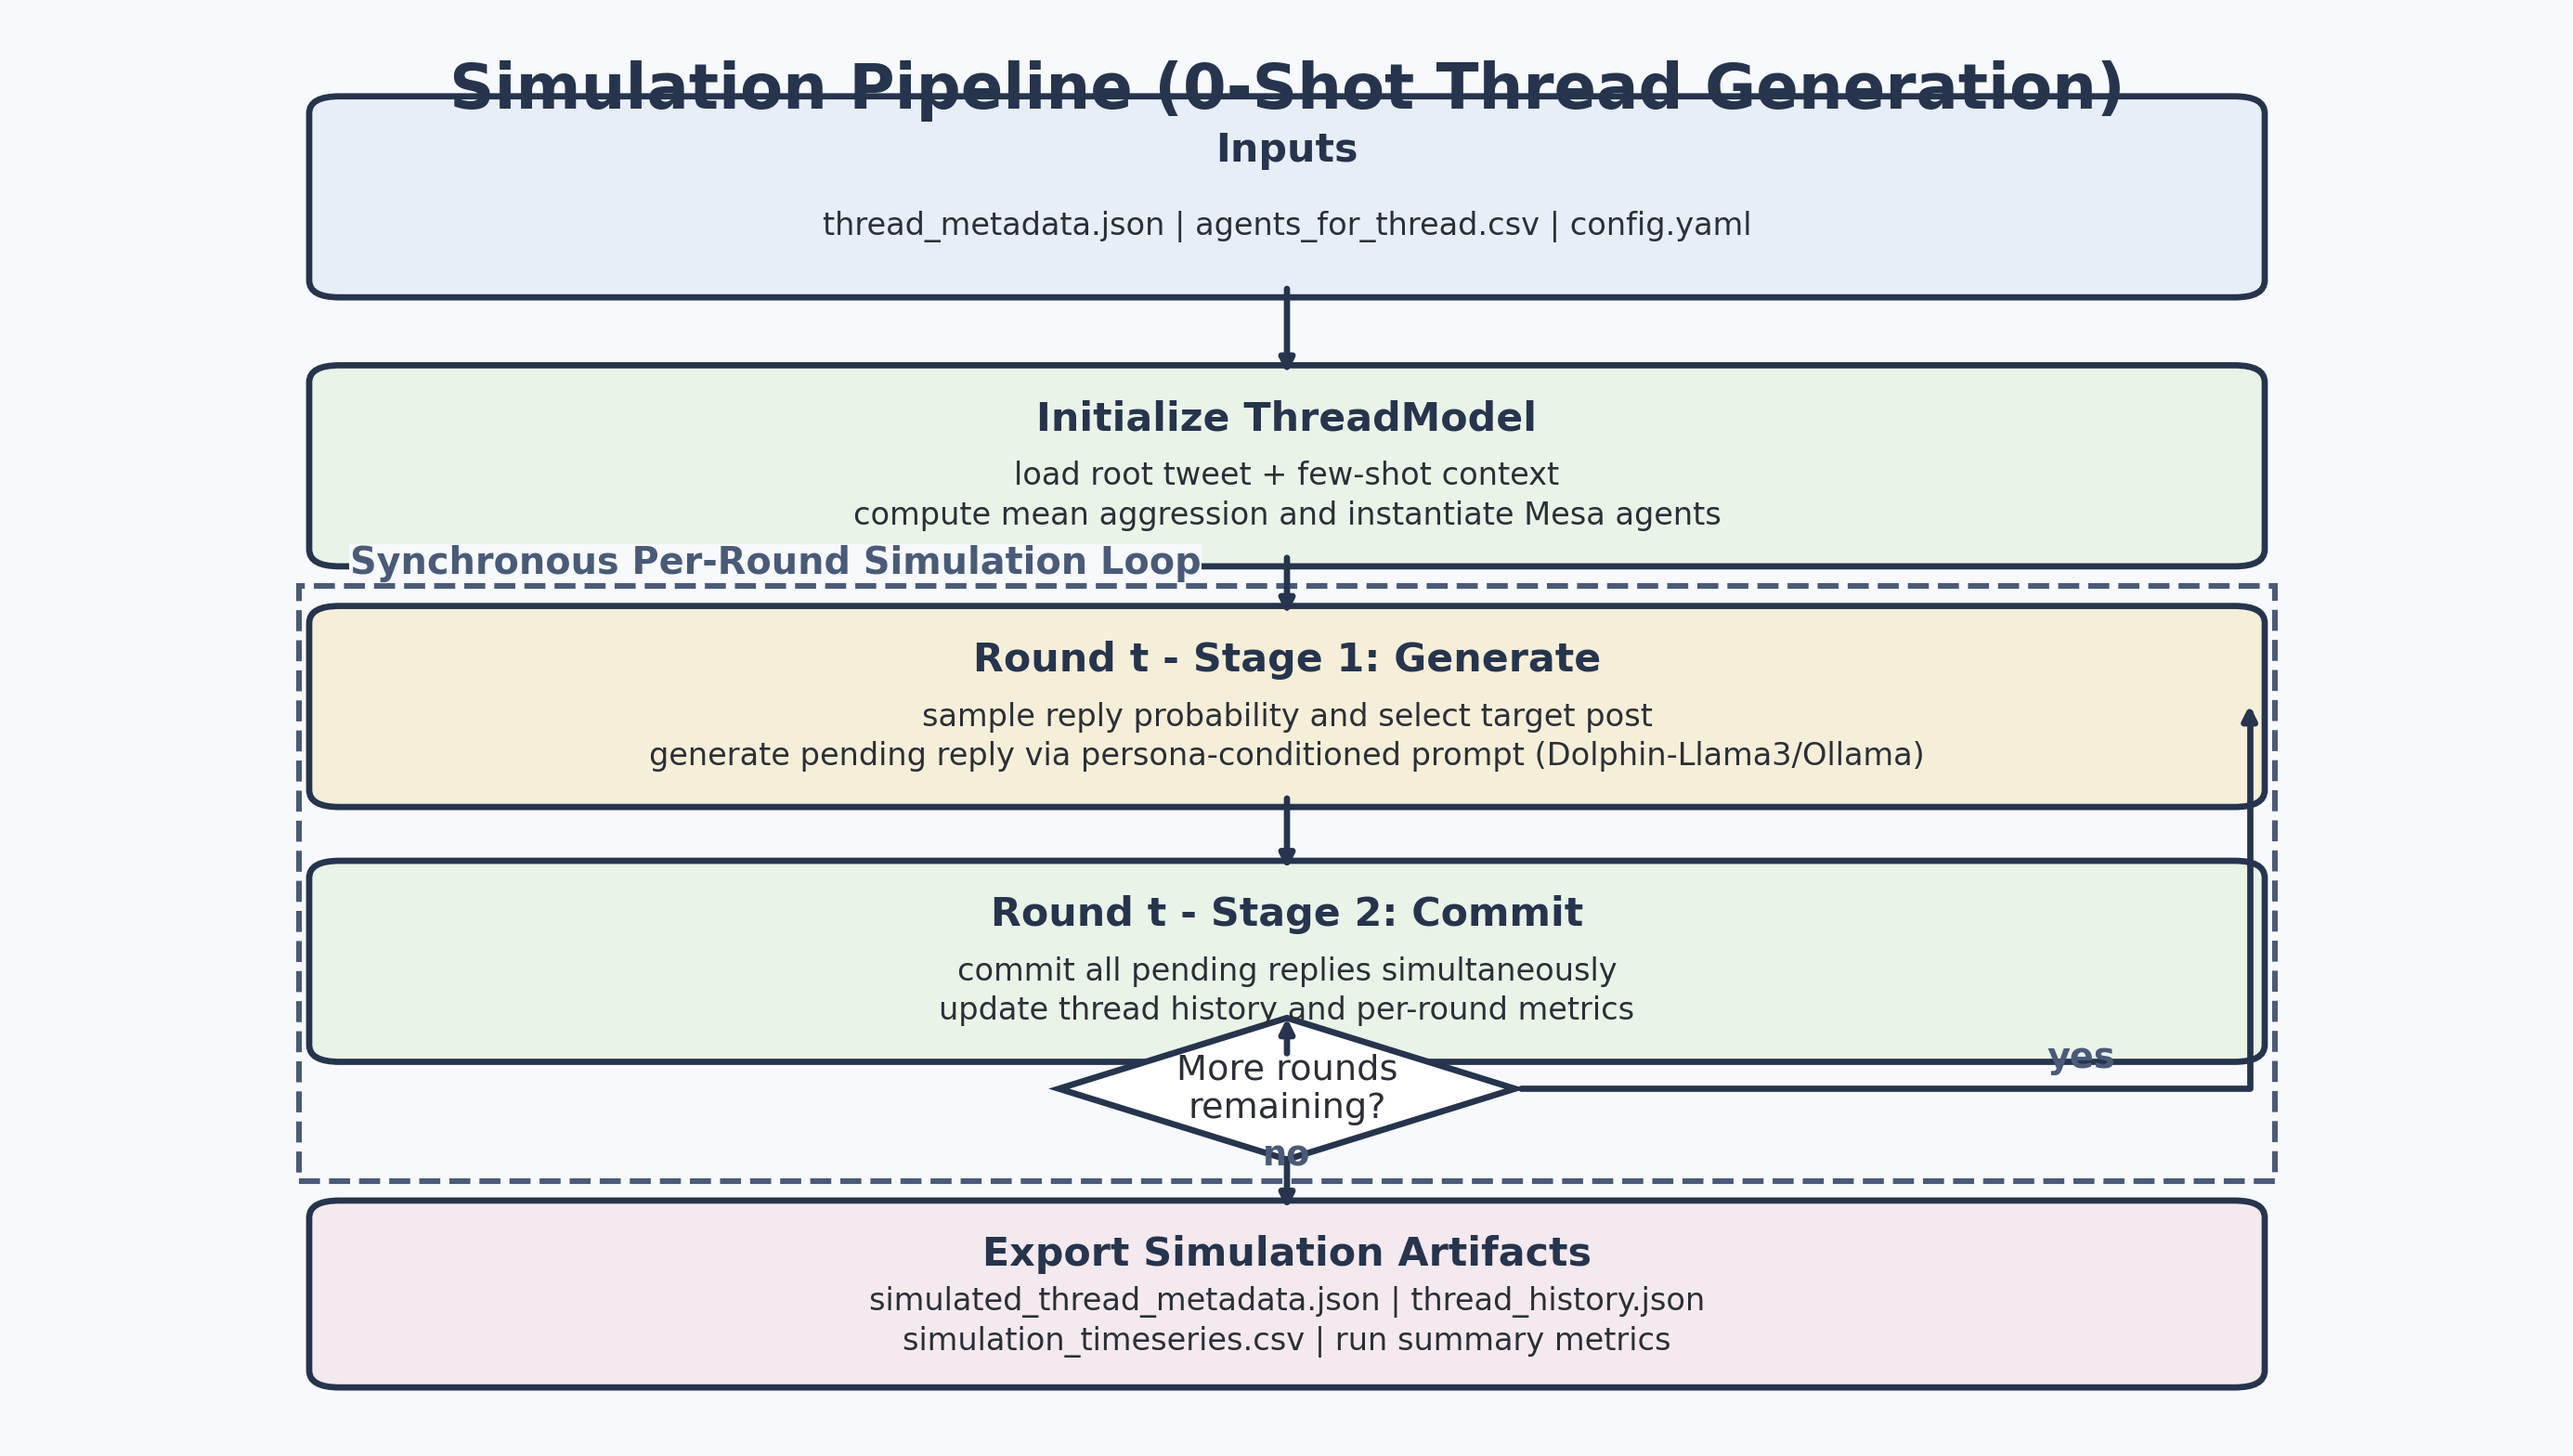
\includegraphics[width=\textwidth]{dissertation_figures/final/02_simulation_pipeline.png}
\caption{Simulation pipeline used in the final system. Agents initialise from the root tweet and configuration files, then iterate through synchronous generate and commit stages before exporting thread-level artefacts.}
\label{fig:simulation_pipeline}
\end{figure}

\section{Phase 1: Initial Prototype Using a General-Purpose Language Model}

The initial approach used a single general-purpose large language model, Anthropic's Claude Haiku (\texttt{claude-haiku-4-5-20251001}), to perform all three pipeline stages: classifying tweet content into agent personality profiles, generating synthetic agent responses, and evaluating the resulting simulated threads. Approximately one million tweets from the USC X 24 dataset were submitted to the Claude API for classification in a single pass, yielding a set of agent personality profiles that included political orientation and inferred behavioural tendencies. These profiles were then used to initialise a set of synthetic agents, which were exposed to high-engagement tweets and prompted to generate responses.

This prototype was identified as fundamentally inadequate upon comparison with real thread data. Across three separate experiments, no agent changed its opinion following any interaction --- opinion scores were identical before and after every simulated exchange. Engagement was minimal, with only two comments generated across the full set of experiments, and no nested reply chains formed at any depth. More critically, the simulated outputs bore no resemblance to the discourse patterns observed in the real threads. The core problem was Claude's reinforcement learning from human feedback (RLHF) alignment, which conditions the model to produce measured, diplomatic, and politically neutral responses. Real political discourse on Twitter/X is characterised by hostility, partisan attack language, and emotional intensity~\citep{brady2017emotion,antypas2023negativity}. A model trained to avoid producing such content cannot serve as a realistic agent in a simulation of that environment, regardless of how the prompt is structured.

These failures motivated a complete redesign of all three pipeline components.

\section{Phase 2: Agent Classification with Specialised Twitter Models}

\subsection{Model Selection}

The classification stage was redesigned to use five specialised transformer models, each trained on large corpora of Twitter/X data and each targeting a distinct dimension of agent behaviour. We rejected general-purpose language models here because political social-media discourse contains abbreviations, hashtags, irony, and coded language that differ materially from the text distributions on which general-purpose models are mainly trained~\citep{antypas2023negativity,tun2023sentiment}. The trade-off is a more complex model stack, but the gain is much stronger domain fit at the point where agent profiles are created.

The five models selected were:

\begin{enumerate}
\item \textbf{Political Leaning} (matous-volf/political-leaning-politics): classifies text as Left, Centre, or Right along the US political spectrum. Trained on twelve US political datasets spanning news articles, social media posts, and political speeches, achieving an F1 score of 83.6\%. This model was selected over alternatives --- including a SemEval 2016 Hillary Clinton stance detection model tested during development --- because it directly measures ideological position rather than sentiment polarity toward a specific politician.
\item \textbf{Emotion} (cardiffnlp/twitter-roberta-base-emotion): classifies the dominant emotional register of a tweet (anger, joy, sadness, fear, etc.), trained as part of the TweetEval benchmark suite.
\item \textbf{Sentiment} (cardiffnlp/twitter-roberta-base-sentiment-latest): classifies overall sentiment as positive, neutral, or negative. Used both during classification and as the primary validation metric.
\item \textbf{Hate Speech} (cardiffnlp/twitter-roberta-base-hate-latest): outputs a continuous hate speech likelihood score normalised to $[0, 1]$.
\item \textbf{Offensive Language} (cardiffnlp/twitter-roberta-base-offensive): outputs a continuous offensiveness score normalised to $[0, 1]$.
\end{enumerate}

Models 2--5 belong to the CardiffNLP Twitter-RoBERTa family, trained on 124 million tweets collected between 2018 and 2021 and evaluated as part of the TweetEval benchmark~\citep{barbieri2020tweeteval}. We sum the hate and offensive scores into a single aggression parameter for the simulation stage. That simplification loses some nuance between targeted hate and general offensiveness, but it gives a usable scalar control signal for reply probability and tone calibration.

\subsection{The Hillary Stance Model Failure}

During development, an initial attempt was made to use cardiffnlp/twitter-roberta-base-stance-hillary (trained for SemEval 2016) as the political orientation classifier. This produced heavily skewed outputs: 68.4\% of users were classified as AGAINST, 30.6\% as NONE, and only 1.1\% as FAVOUR, despite the underlying dataset containing 2.5 times more Biden mentions than Trump mentions. Investigation revealed that the model detects sentiment polarity toward Hillary Clinton specifically rather than general political ideology --- the majority of political tweets are negative in tone regardless of which side of the debate they occupy, causing the model to classify most content as AGAINST. The Hillary model was replaced with the political leaning classifier described above, which directly measures ideological position and produced distributions consistent with broader survey patterns of Twitter/X user behaviour~\citep{smith2021twitterbehaviors,smith2022politicalcontent}.

This failure exposed a broader design rule for the dissertation: domain-specific models still require task-specific validation. We therefore made raw-output inspection and distribution checks mandatory before adopting any classifier in the pipeline.

\subsection{User-Level Aggregation}

Classification was performed at the tweet level, then aggregated to the user level to produce agent DNA profiles. We made that choice because agents represent users, not individual tweets. Over the sampled period, we treat each user's tweets as noisy observations of a relatively stable behavioural profile. Mean scores are taken for continuous variables (political score, emotion score, sentiment score, hate, offensive), dominant labels by mode for categorical variables (political leaning, dominant emotion, dominant sentiment), and total engagement by summation. This produces one profile row per user and keeps the simulator tied to historical personas rather than isolated posts.

\subsection{Infrastructure}

Classification was performed on Google Cloud Platform virtual machine instances equipped with NVIDIA Tesla T4 GPUs. All five models were loaded in a single pass per chunk of data, processing approximately 50,000 tweets per chunk. A checkpoint system saved progress every 1,000 tweets, enabling recovery from interruptions without reprocessing completed work.

\section{Phase 3: Discourse Simulation with an Uncensored Language Model}

\subsection{The Censorship Problem}

Having established a validated agent classification pipeline, the simulation stage required a language model capable of generating realistic political Twitter discourse. Claude Haiku (\texttt{claude-haiku-4-5-20251001}) was re-evaluated in this role and found to produce outputs that were overwhelmingly positive in sentiment (84.8\% positive) when real threads of the same type are predominantly negative. Prompt engineering alone was unable to overcome this limitation: RLHF safety alignment is applied during fine-tuning and cannot be removed through instruction. The simulation requires a model that can produce the hostile, partisan, emotionally intense language that characterises real political discourse~\citep{brady2017emotion,antypas2023negativity,tun2023sentiment}.

\subsection{Model Selection: Dolphin-Llama3 8B}

We selected Dolphin-Llama3 8B as the simulation model because the main failure of aligned models in this task is not fluency but tone suppression. Dolphin-Llama3 8B is an uncensored fine-tune of Meta's Llama 3 architecture produced by Eric Hartford, with the RLHF safety constraints relaxed so that the model can generate the hostile and partisan language that aligned models often refuse to produce. The trade-off is obvious: looser safety controls require tighter research handling. For that reason, all generation remained in a closed research environment. The model was deployed locally via Ollama on the GCP T4 instance, which also made iterative tuning in Phase~5 practical.

\subsection{Agent Architecture and Simulation Logic}

Agents were implemented using the Mesa agent-based modelling framework. Each agent was initialised with the DNA profile derived from Phase 2: political leaning, dominant emotion, sentiment, and an aggression score. At each simulation step, agents probabilistically decided whether to post a reply, with base probability of 5\% modified upward by the agent's aggression score. Agents with high aggression scores were more likely to engage and more likely to target ideologically opposing agents, consistent with the Backfire Effect described in the theoretical framework~\citep{diehl2016political,brady2017emotion,composta2025simulating}.

Each agent's system prompt was constructed from its DNA profile, translating categorical labels into behavioural descriptions. Political orientation was described in terms of values and vocabulary rather than labels --- Left-leaning agents were instructed to support social justice and government accountability; Right-leaning agents to support limited government and traditional values --- because small language models (8B parameters) tend to echo categorical labels rather than embody them, producing outputs that explicitly identify themselves as ``a Left-leaning Twitter user'' rather than generating authentic partisan content ~\citep{park2023generative}. Aggression was mapped to one of five tone tiers, ranging from ``casual and conversational'' for agents below 0.15 to ``confrontational'' for agents above 0.7.

The simulation proceeded for ten rounds, with reply decisions and pending generations evaluated against a shared thread state before any new replies were committed, preventing sequential activation bias. Output was stored in a structured JSON format matching the real thread metadata schema, enabling direct comparison by the validation framework.

\section{Phase 4: Validation Framework}

\subsection{Design Rationale}

Validation had to answer a stricter question than ``does the text look plausible?'' It had to determine whether independently generated synthetic threads match real ones closely enough to be useful as a research instrument. Jensen--Shannon Divergence (JSD) was chosen as the primary comparison metric because it is symmetric, bounded on $[0, 1]$, and well-defined even when the two distributions assign zero probability to different categories. A JSD of 0 indicates identical distributions; in this dissertation, values below 0.15 are treated as good similarity.

\subsection{Multidimensional Validation}

Initial validation used a single dimension, sentiment, and reported a high accuracy score that later proved misleading. Once we expanded evaluation to five dimensions --- sentiment, political leaning, emotion distribution, aggression level, and keyword content --- the early simulation was shown to produce politically inverted output, near-zero aggression, and replies in which the model identified itself as an AI. Sentiment alone could not detect these failures because a thread can match negative/neutral/positive proportions while still being wrong in politics, tone, and interaction style.

The five-dimensional validation framework classified every generated tweet through the same five RoBERTa models used in the classification stage, ensuring methodological consistency and eliminating the need for an external oracle. JSD was computed for the sentiment, political, and emotion distributions. A continuous sentiment score was extracted by computing $P(\text{positive}) - P(\text{negative})$ from the model's raw probability outputs, enabling paired statistical testing across threads~\citep{antypas2023negativity,tun2023sentiment}.

\subsection{Statistical Testing}

To determine whether any systematic bias existed between simulated and real thread sentiment, a Wilcoxon signed-rank test was applied to the per-thread mean sentiment scores (real vs.\ simulated). This non-parametric test was chosen because the distribution of sentiment differences across threads cannot be assumed to be normal. A statistically significant result ($p < 0.05$) indicates that the simulation exhibits a consistent directional bias; a non-significant result indicates that any differences are indistinguishable from random variation.

\section{Phase 5: Parameter Optimisation}

\subsection{Initial Parameter Failure}

A preliminary 100-thread batch validation, run to test whether the redesigned pipeline was viable, revealed its main remaining defect: systematic negative sentiment bias. The mean per-thread sentiment residual (simulated minus real, on a $[-1, +1]$ scale) was $-0.390 \pm 0.196$, and the Wilcoxon test confirmed that this bias was not random ($p = 4.27 \times 10^{-18}$). In other words, the system was consistently producing more hostile and negative content than the real threads it was meant to simulate. Political distribution and output volume were broadly reasonable, but emotional calibration was still wrong.

Root cause analysis identified several compounding issues. The system prompt instructed all agents to ``match the hostility level of the thread --- Political Twitter is aggressive,'' which imposed a global negativity floor that overrode per-agent aggression calibration. The aggression tier descriptions used extreme language at all levels, meaning even low-aggression agents were instructed to be combative.

\subsection{Prompt Engineering Fixes}

Four coordinated changes were made to address the identified failures:

\begin{enumerate}
\item \textbf{Softened aggression tone tiers}: The four-tier aggression system was expanded to five tiers and the most extreme language removed. A new lowest tier (aggression $< 0.15$) explicitly permitted casual, conversational, and even agreeable replies, giving the model permission to generate non-negative content for low-aggression agents.
\item \textbf{Rule 6 replacement}: The global hostility instruction (``Political Twitter is aggressive'') was replaced with ``Not every reply is an attack. Sometimes you agree with someone, crack a joke, share a fact, or express genuine concern. Vary your tone naturally.'' This removed the negativity floor that was overriding per-agent calibration.
\item \textbf{Dynamic aggression scaling}: Agent aggression tiers were computed relative to the thread's mean aggression rather than against absolute thresholds. An agent at aggression 0.35 in a mild thread (mean 0.15) was assigned a more assertive tone; the same agent in a hostile thread (mean 0.50) was assigned a calmer tier. This introduced thread-level sensitivity into agent behaviour.
\item \textbf{Expanded context window}: The number of recent posts in the simulation shown to each agent as conversational context was increased from 3 to 8, providing a more representative sample of the thread's current tone.
\end{enumerate}

\subsection{Zero-Shot Prompting}

All simulations in this dissertation were run in 0-shot mode: no real reply texts from the target thread were provided to the LLM at generation time. This constraint is methodological, not incidental. It ensures that strong results reflect forward simulation rather than hidden target-thread leakage. Prompt engineering therefore focused only on changes compatible with that constraint, including calibrated aggression tiers, revised behavioural instructions, dynamic aggression scaling, context-window expansion, and vocabulary injection.

\section{Phase 6: Ablation Study}

To identify which design choices most contributed to simulation quality, we conducted a systematic ablation study in 0-shot mode across 21 parameter configurations, each run across 10 diverse threads from the USC dataset (210 total simulations). The 0-shot constraint was imposed deliberately so every configuration was tested under the same forward-only conditions. Configurations were constructed as single-parameter ablations from the 0-shot baseline --- changing exactly one parameter at a time --- plus five multi-parameter combinations designed to test specific interaction hypotheses.

Parameters varied included: temperature (0.7, 0.9, 1.2), context window size (3, 8, 15 posts), dynamic aggression scaling (on/off), the Rule 6 formulation (permissive vs.\ hostile), aggression tier count (4 vs.\ 5 tiers), reply probability (2\%, 5\%, 10\%), controversy targeting weight (1.0, 2.5, 5.0), vocabulary injection (on/off), repeat penalty (1.1, 1.3), response length (80 vs.\ 150 tokens), and simulation length (10 vs.\ 20 rounds).

The 0-shot baseline (with vocabulary injection retained) achieved the highest composite score (0.780). Removing vocabulary injection degraded performance substantially (rank 16, score 0.548), confirming that the politically charged keyword banks help anchor agent language to authentic partisan discourse. The most impactful positive single-parameter changes were expanding the context window from 8 to 15 posts (rank 6, score 0.713) and increasing temperature from 0.9 to 1.2 (rank 7, score 0.694). The most impactful negative changes were increasing repeat penalty to 1.3 (score 0.429), extending simulation length to 20 rounds (score 0.411), and reducing temperature to 0.7 (score 0.451).

Reply probability was also an influential parameter: halving the base probability from 5\% to 2\% produced the second-best configuration (score 0.777), because lower participation concentrated output among the most motivated agents, improving lexical realism and reducing redundancy. Conversely, doubling reply probability to 10\% improved political alignment but degraded lexical diversity and stance consistency.

The final 100-thread simulation runs reported in the Results section used the optimised 0-shot parameter set, including vocabulary injection, as these produced the best overall results in pipeline validation.

% ==========================================
% CHAPTER 5: EVALUATION
% ==========================================
\chapter{Evaluation}

\section{Overview}

Across 100 held-out threads, the final pipeline reaches mean overall accuracy of $92.3\% \pm 4.6\%$ and composite fidelity of $0.857 \pm 0.106$, with no significant directional sentiment bias. This chapter explains that result in three stages. Section~\ref{sec:100thread} reports the full 100-thread validation run and establishes where the system matches real discourse well and where it fails. Section~\ref{sec:fidelity} then compresses per-thread performance into a composite fidelity score so that the distribution of outcomes can be analysed directly. Section~\ref{sec:ablation_eval} uses the 21-configuration ablation study to show which design choices matter most for fidelity, before the discussion section interprets what the pipeline is actually useful for.

All evaluation was performed against ground-truth data from the USC~X~24 dataset. Simulated threads were generated from the root tweet and agent DNA profiles in 0-shot mode, with no injected real reply texts from the target thread. The simulation did not have access to the full set of real thread replies or to the validation metrics of the target thread.

% ------------------------------------------
\section{100-Thread Validation}
\label{sec:100thread}

The optimised pipeline (0-shot parameters with vocabulary injection) was run across 100 threads drawn from the USC~X~24 dataset. All 100 simulations completed successfully with no failures. The corpus comprised 6,528 real tweets and 6,097 simulated tweets (12,625 total), with threads ranging from 15 to 124 simulated posts.

\subsection{Distributional Similarity}

Three Jensen--Shannon Divergence (JSD) metrics were computed per thread, comparing the simulated and real distributions of sentiment, political leaning, and emotion labels. Table~\ref{tab:jsd_results} summarises the results.

\begin{table}[ht]
\centering
\caption{JSD between simulated and real distributions across 100 threads.}
\label{tab:jsd_results}
\begin{tabular}{lcc}
\toprule
\textbf{Dimension} & \textbf{Mean JSD} & \textbf{Std Dev} \\
\midrule
Sentiment   & 0.086 & 0.079 \\
Political   & 0.039 & 0.038 \\
Emotion     & 0.118 & 0.105 \\
\bottomrule
\end{tabular}
\end{table}

All three mean JSD values fall below the 0.15 threshold adopted for good distributional similarity. Political leaning is the best-matched dimension (mean JSD~$= 0.039$), indicating that the simulation accurately reproduces the partisan composition of real threads. Sentiment alignment is strong (mean JSD~$= 0.086$), and emotion is the most variable dimension (mean JSD~$= 0.118$), reflecting the greater difficulty of matching fine-grained emotional registers~\citep{antypas2023negativity,brady2017emotion}.

Figure~\ref{fig:jsd_boxplot} shows the per-thread JSD distributions as box plots. The political JSD is tightly concentrated near zero with few outliers; sentiment and emotion exhibit longer tails corresponding to threads where the simulation diverged from the real distribution.

\begin{figure}[ht]
\centering
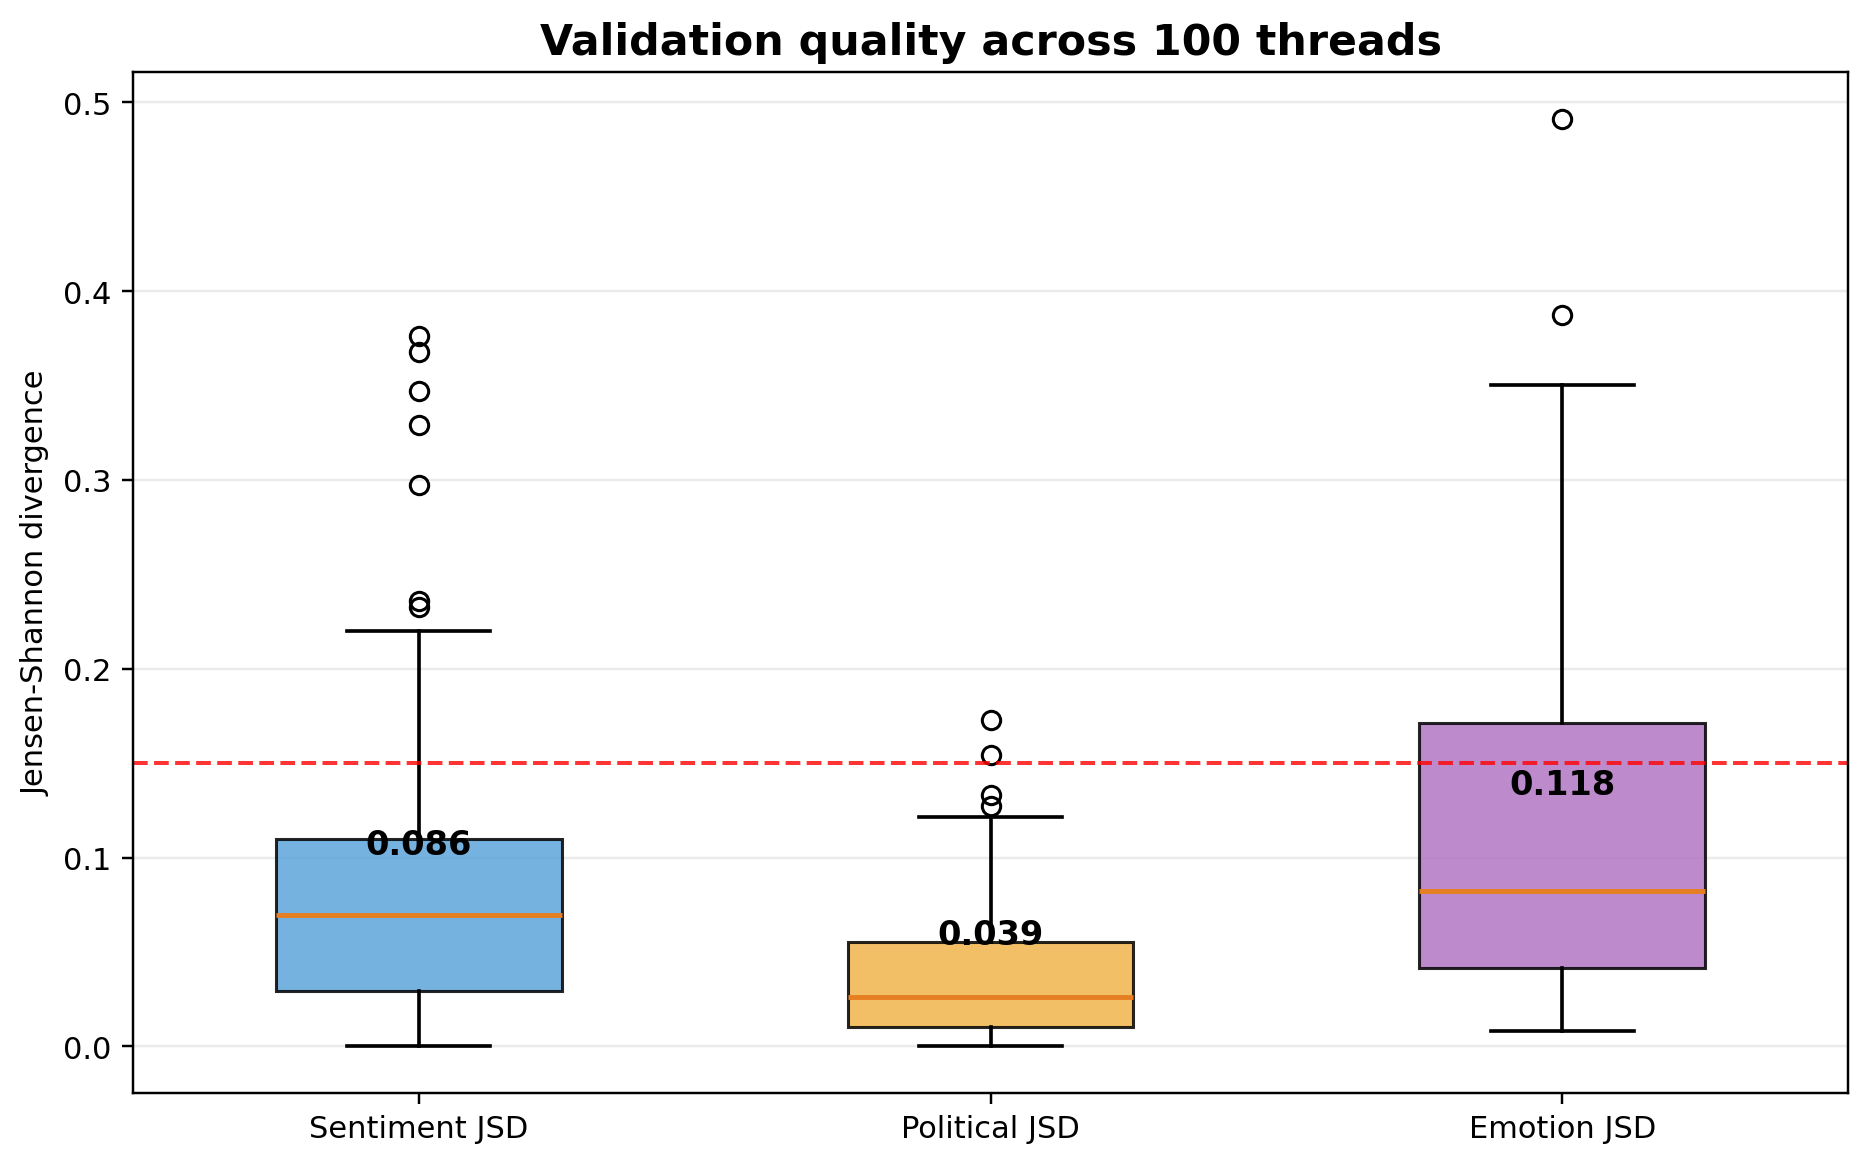
\includegraphics[width=0.85\textwidth]{dissertation_figures/final/03_jsd_boxplot.png}
\caption{JSD distributions across 100 threads for sentiment, political leaning, and emotion. The red dashed line marks the JSD = 0.15 reference threshold used in the analysis.}
\label{fig:jsd_boxplot}
\end{figure}

\subsection{Sentiment Bias Analysis}

A critical requirement of the simulation is the absence of systematic directional bias. The mean per-thread sentiment residual (simulated mean minus real mean, on a $[-1, +1]$ scale) was $+0.025 \pm 0.351$. The Wilcoxon signed-rank test yielded $W = 2386.0$, $p = 0.633$, indicating that the observed residuals are statistically indistinguishable from zero. The simulation does not exhibit a systematic tendency to produce more positive or more negative content than the real threads.

This result represents a substantial improvement over the initial pipeline, which exhibited a mean residual of $-0.390$ and a Wilcoxon $p = 4.27 \times 10^{-18}$ (Section~4.5.1). The prompt engineering changes described in Section~4.5.2 successfully eliminated the systematic negative bias.

\begin{figure}[ht]
\centering
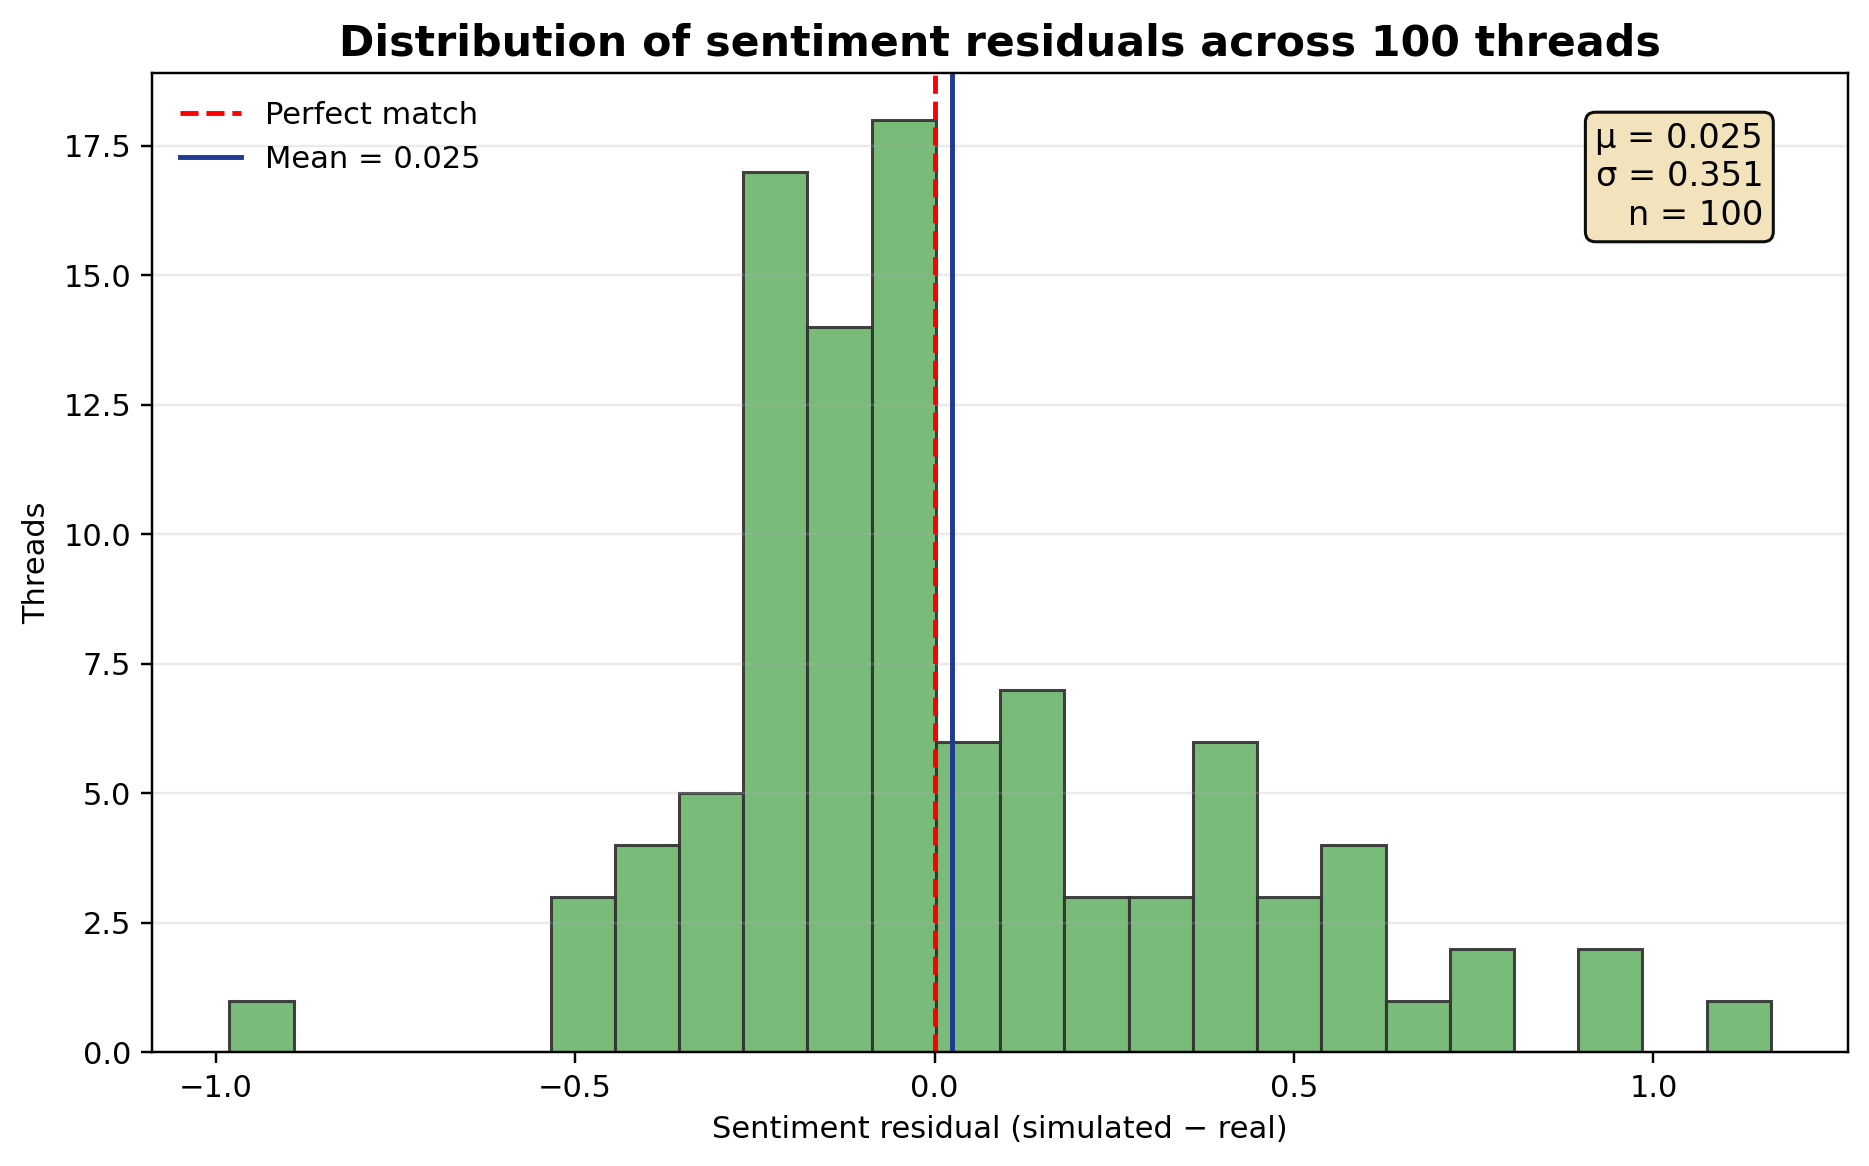
\includegraphics[width=0.85\textwidth]{dissertation_figures/final/04_sentiment_residual_histogram.png}
\caption{Distribution of per-thread sentiment residuals (simulated $-$ real). The distribution is centred near zero, confirming the absence of systematic bias.}
\label{fig:sentiment_residual}
\end{figure}

\subsection{Aggression Calibration}

The Pearson correlation between real and simulated mean aggression scores across threads was $r = 0.332$, $p < 0.001$. While this represents a statistically significant positive correlation --- threads with more aggressive real participants produce more aggressive simulated output --- the moderate effect size indicates room for improvement in fine-grained hostility calibration.

\begin{figure}[ht]
\centering
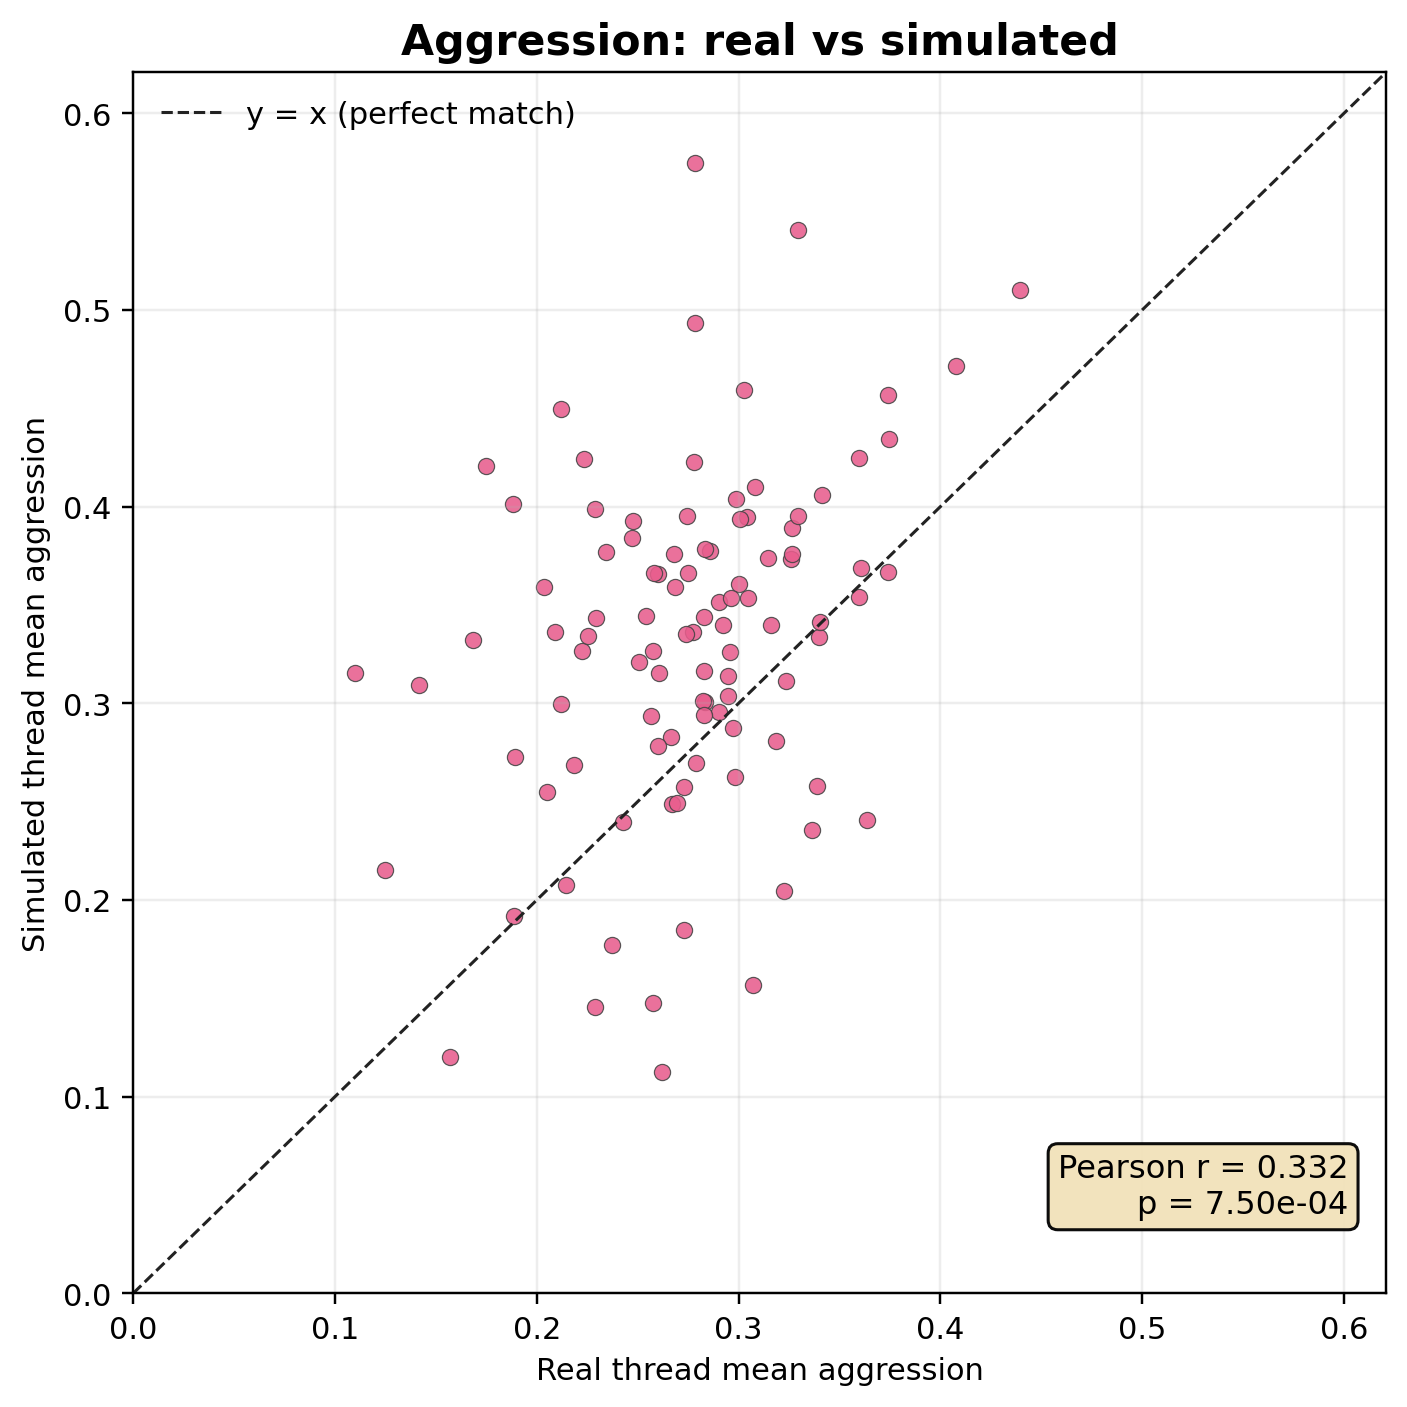
\includegraphics[width=0.75\textwidth]{dissertation_figures/final/05_aggression_scatter.png}
\caption{Scatter plot of real vs.\ simulated mean aggression per thread. The positive correlation ($r = 0.332$) confirms that the simulation's hostility level tracks real thread aggression.}
\label{fig:aggression}
\end{figure}

\subsection{Overall Accuracy}

The weighted overall accuracy score (Equation~3.1) was computed per thread. The mean overall accuracy across 100 threads was $92.3\% \pm 4.6\%$. When categorised by accuracy band: 97 threads were rated EXCELLENT ($\geq 80\%$), 3 were rated GOOD (60--79\%), and none were rated FAIR or POOR. Note that this overall accuracy metric (Equation~3.1) differs from the composite fidelity score introduced in Section~\ref{sec:fidelity}, which incorporates additional sub-metrics and uses a different normalisation scheme.

\begin{figure}[ht]
\centering
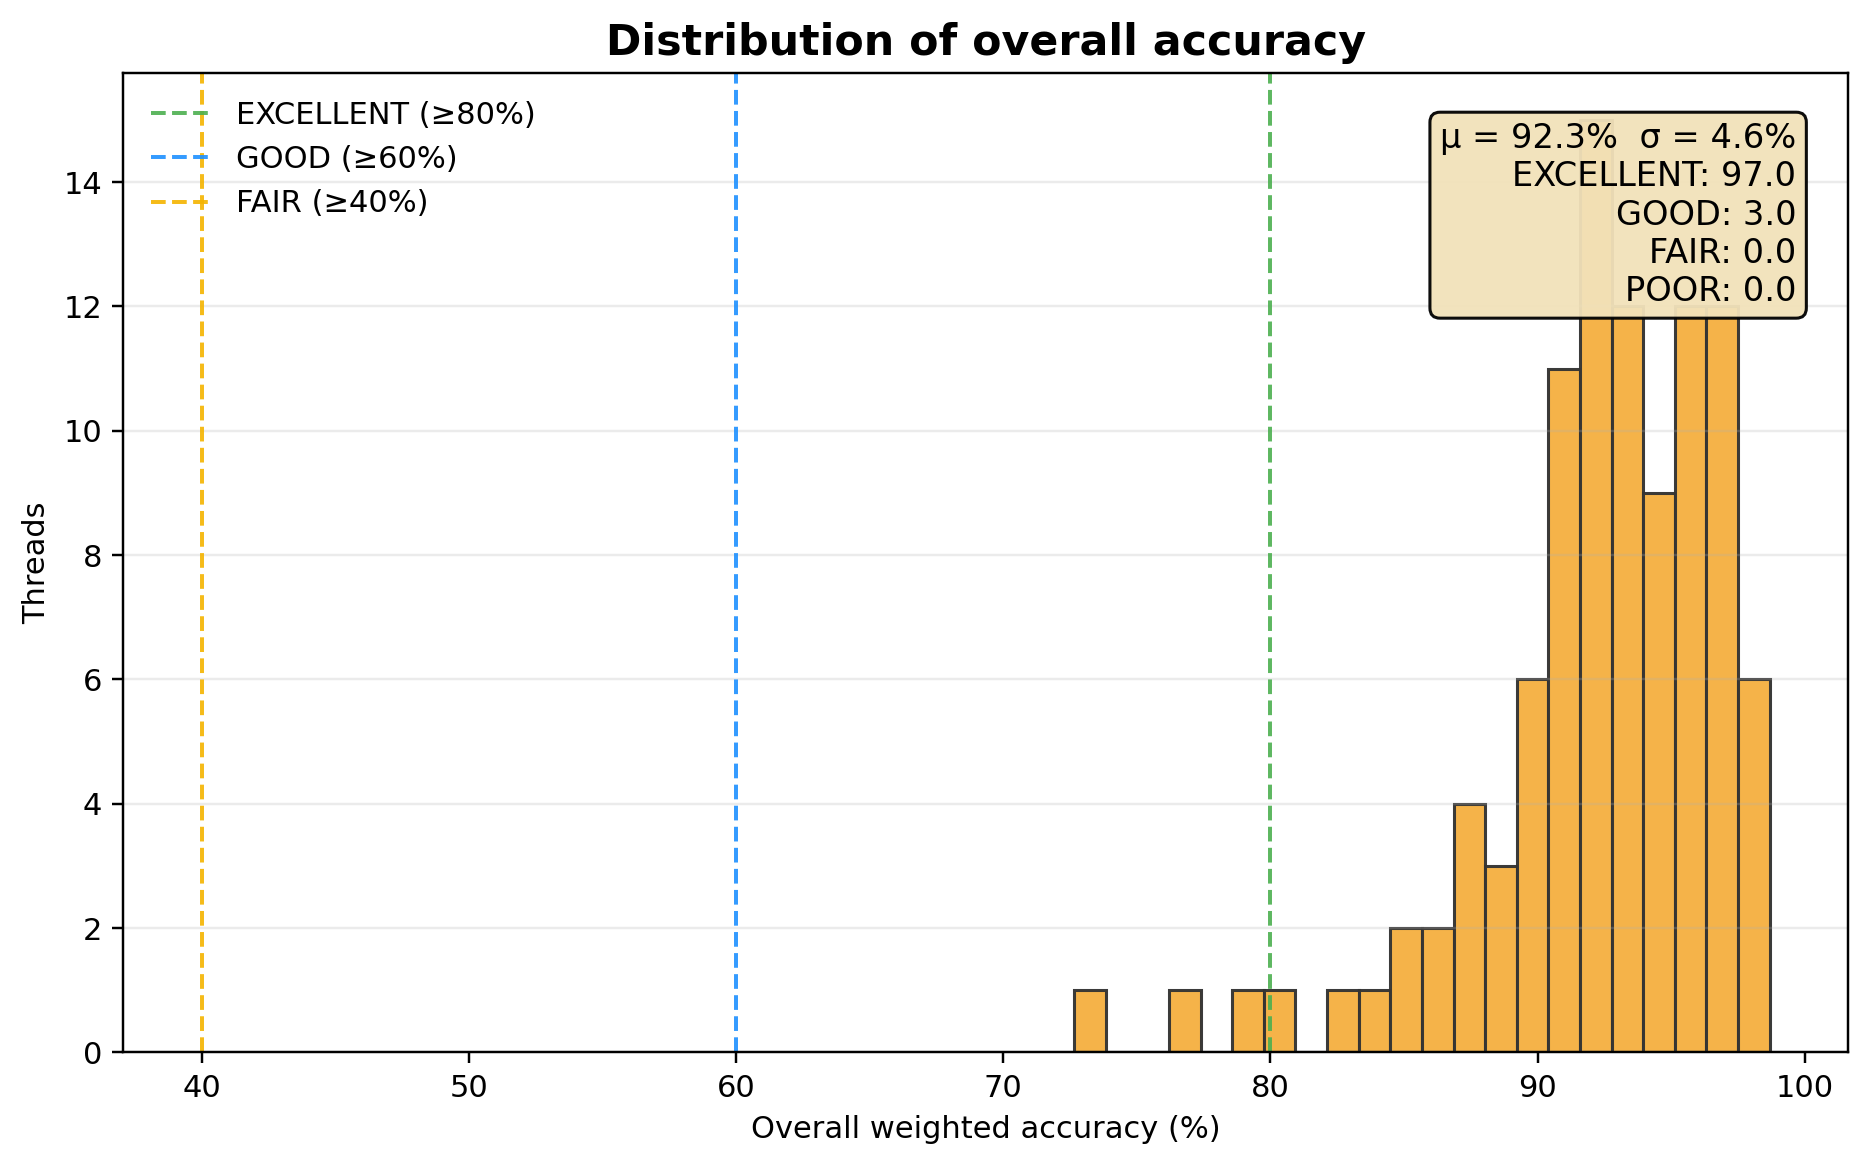
\includegraphics[width=0.85\textwidth]{dissertation_figures/final/06_overall_accuracy_histogram.png}
\caption{Distribution of per-thread overall accuracy scores. The negatively skewed distribution confirms consistently high performance, with 97\% of threads rated EXCELLENT.}
\label{fig:accuracy_hist}
\end{figure}

\subsection{Aggregate Distribution Comparison}

Figure~\ref{fig:political_aggregate} shows aggregate political distributions across all 100 threads, and Figure~\ref{fig:sentiment_overlay} shows the pooled sentiment score distributions. The simulation produces comparable overall discourse volume (6,097 simulated tweets vs 6,528 real tweets) while preserving close distributional alignment at the corpus level.

\begin{figure}[ht]
\centering
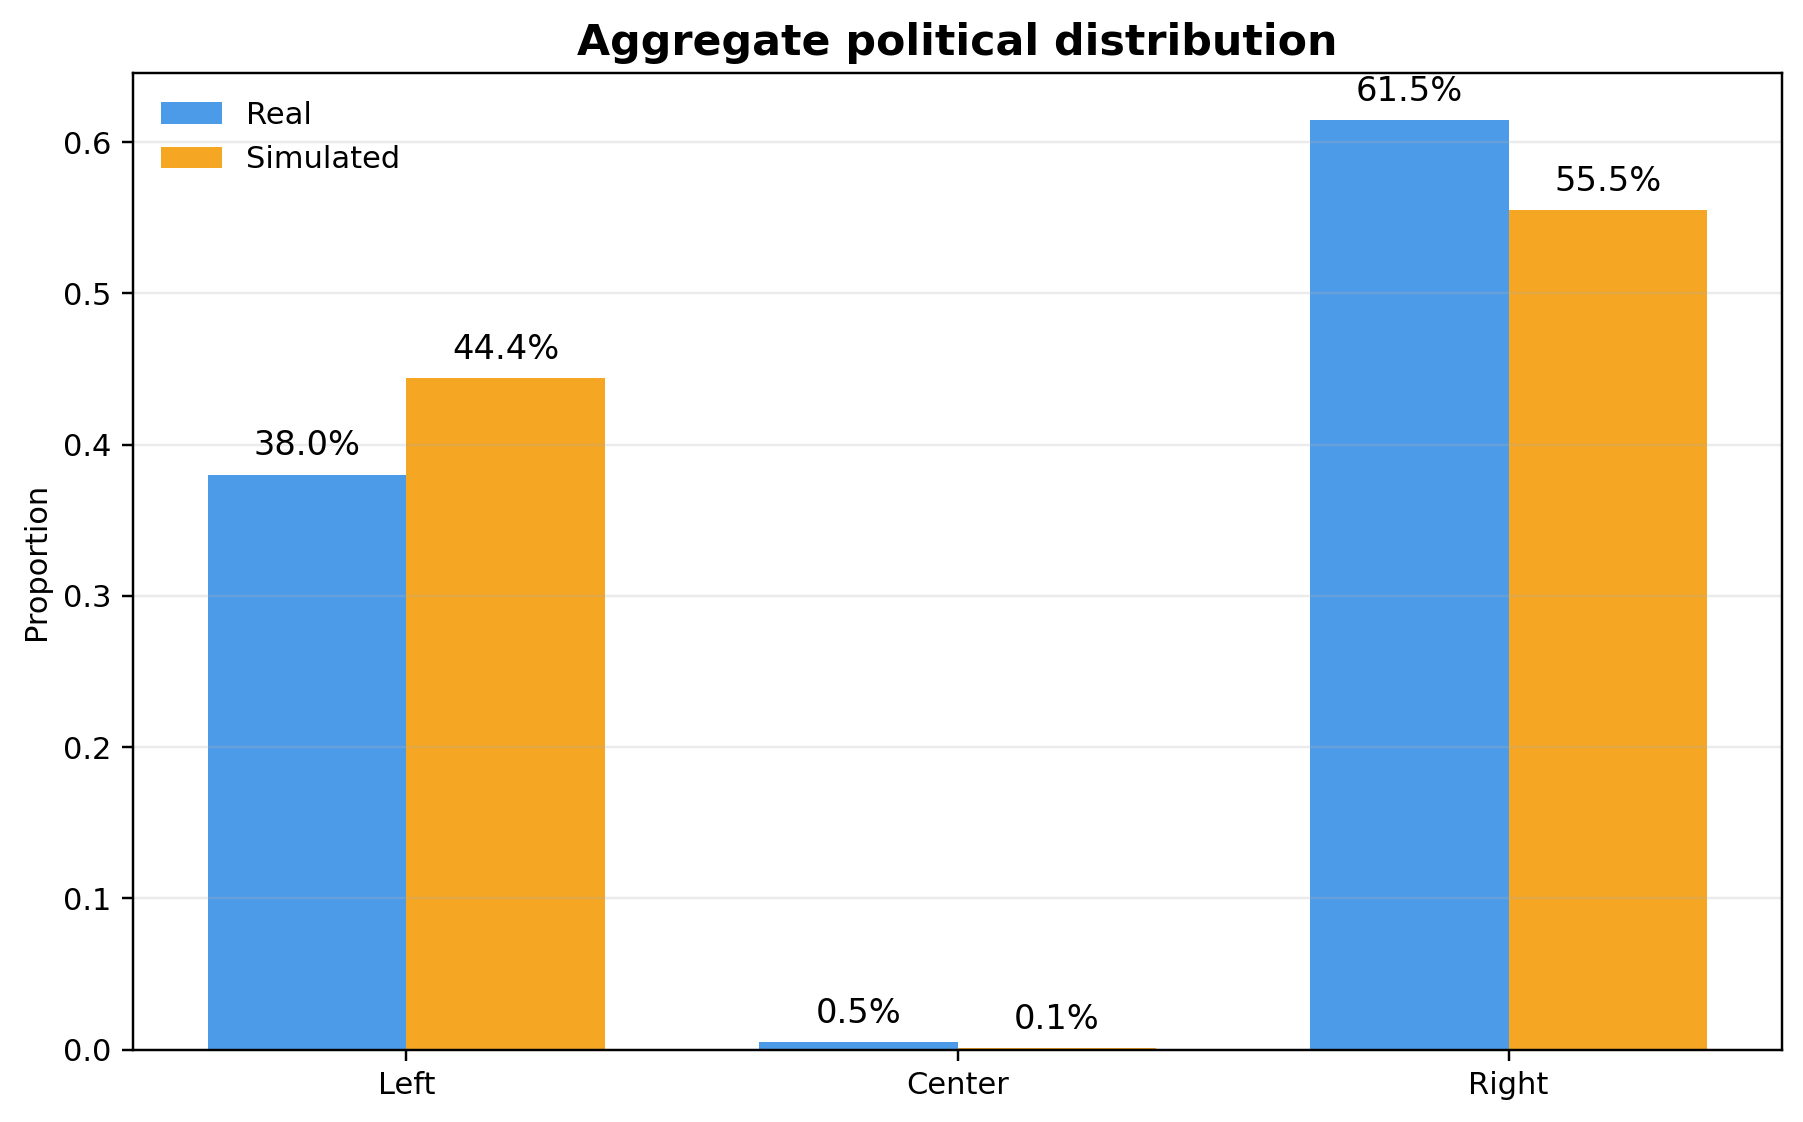
\includegraphics[width=0.85\textwidth]{dissertation_figures/final/07_political_aggregate.png}
\caption{Aggregate political distribution: real vs.\ simulated across all 100 threads. The simulation reproduces the Left/Right split with a slight left-shift at the aggregate level.}
\label{fig:political_aggregate}
\end{figure}

\begin{figure}[ht]
\centering
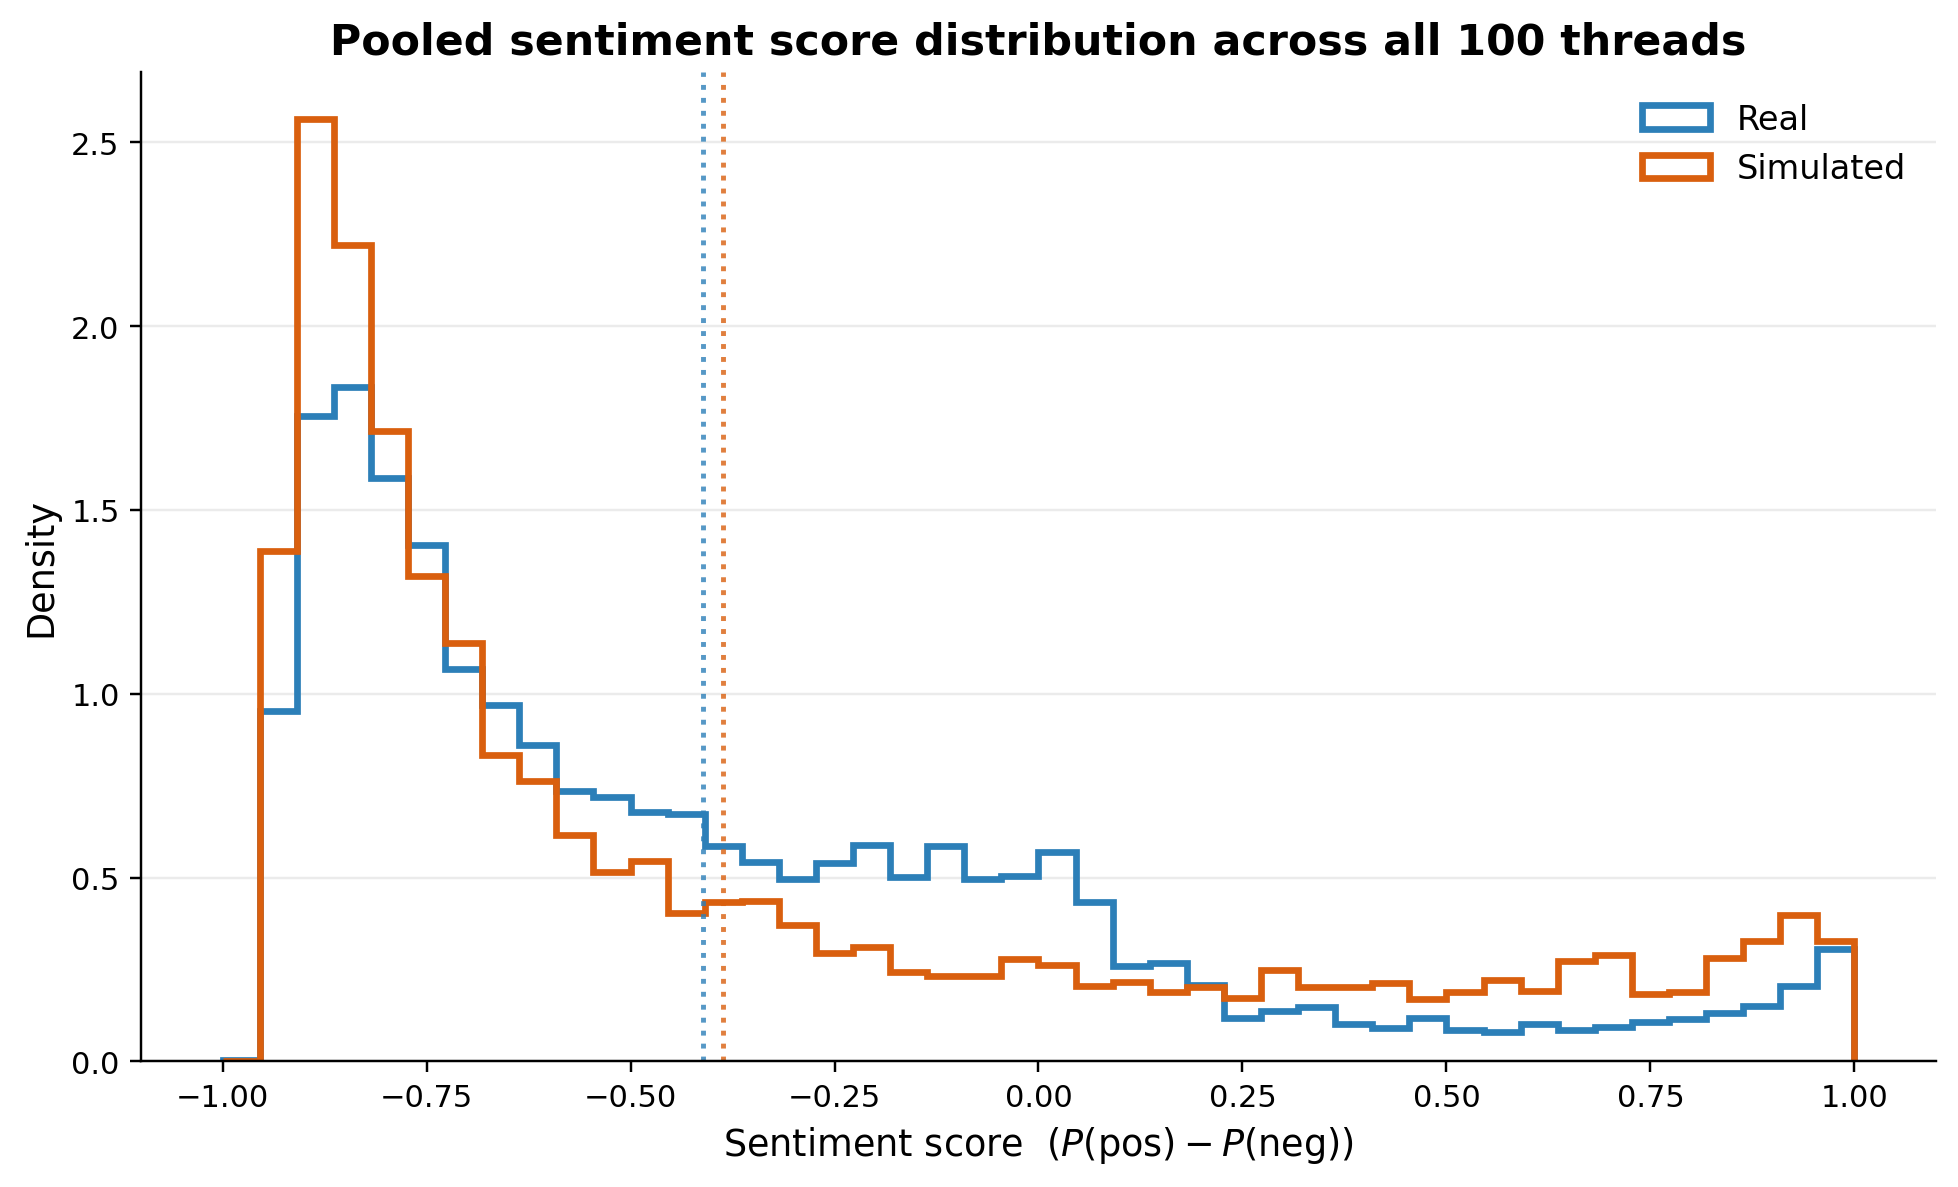
\includegraphics[width=0.85\textwidth]{dissertation_figures/final/08_sentiment_distribution_comparison.png}
\caption{Pooled continuous sentiment-score distributions for real and simulated replies across all 100 threads. Unfilled step histograms are used to preserve visibility in regions of overlap, and dotted lines mark the mean score for each corpus.}
\label{fig:sentiment_overlay}
\end{figure}

% ------------------------------------------
\section{Composite Fidelity Score}
\label{sec:fidelity}

To enable a single-number summary of per-thread simulation quality, a composite fidelity score was constructed as a weighted average of five normalised sub-metrics. Each divergence metric was converted to a $[0, 1]$ fidelity score using $1 - \min(v / c, 1)$, where $v$ is the raw metric value and $c$ is a theoretical upper bound (JSD cap $= \ln 2 \approx 0.693$; sentiment residual cap $= 1.0$). Overall accuracy was normalised by dividing by 100.

The composite score was computed as:
\begin{equation}
\text{Fidelity} = 0.30 \times f_{\text{sent}} + 0.20 \times f_{\text{emo}} + 0.15 \times f_{\text{pol}} + 0.20 \times f_{\text{res}} + 0.15 \times f_{\text{acc}}
\end{equation}
where $f_{\text{sent}}$, $f_{\text{emo}}$, $f_{\text{pol}}$ are the JSD-based fidelity scores for sentiment, emotion, and political leaning respectively, $f_{\text{res}}$ is the absolute sentiment residual fidelity, and $f_{\text{acc}}$ is the normalised overall accuracy.

\subsection{Distribution of Fidelity Scores}

Across 100 threads, the composite fidelity score had a mean of $0.857 \pm 0.106$, with a median of $0.885$. Most threads cluster in the high-fidelity range around 0.80--0.97, with only a small tail of lower-performing cases. Of 100 threads, 45 scored $\geq 0.90$ (excellent fidelity), 79 scored $\geq 0.80$, and only 7 scored below $0.70$.

The best-performing thread (thread\_073, fidelity $= 0.977$) matched the real distribution almost exactly across all five dimensions. The worst-performing thread (thread\_061, fidelity $= 0.431$) exhibited a large sentiment polarity inversion --- the simulation generated predominantly positive content for a thread that was overwhelmingly negative. Sub-metric analysis showed that political JSD fidelity and overall accuracy were consistently high with tight spreads, while absolute sentiment residual varied the most. That makes polarity inversion the dominant failure mode: when a thread's tone is misjudged, the composite score drops sharply.

Figure~\ref{fig:fidelity_ranked} shows all 100 threads ranked by fidelity score, colour-coded by quality tier. The smooth degradation curve confirms that the system does not exhibit bimodal behaviour (i.e., it does not produce either perfect or catastrophic results), but rather degrades gracefully with a long tail of progressively harder threads.

\begin{figure}[ht]
\centering
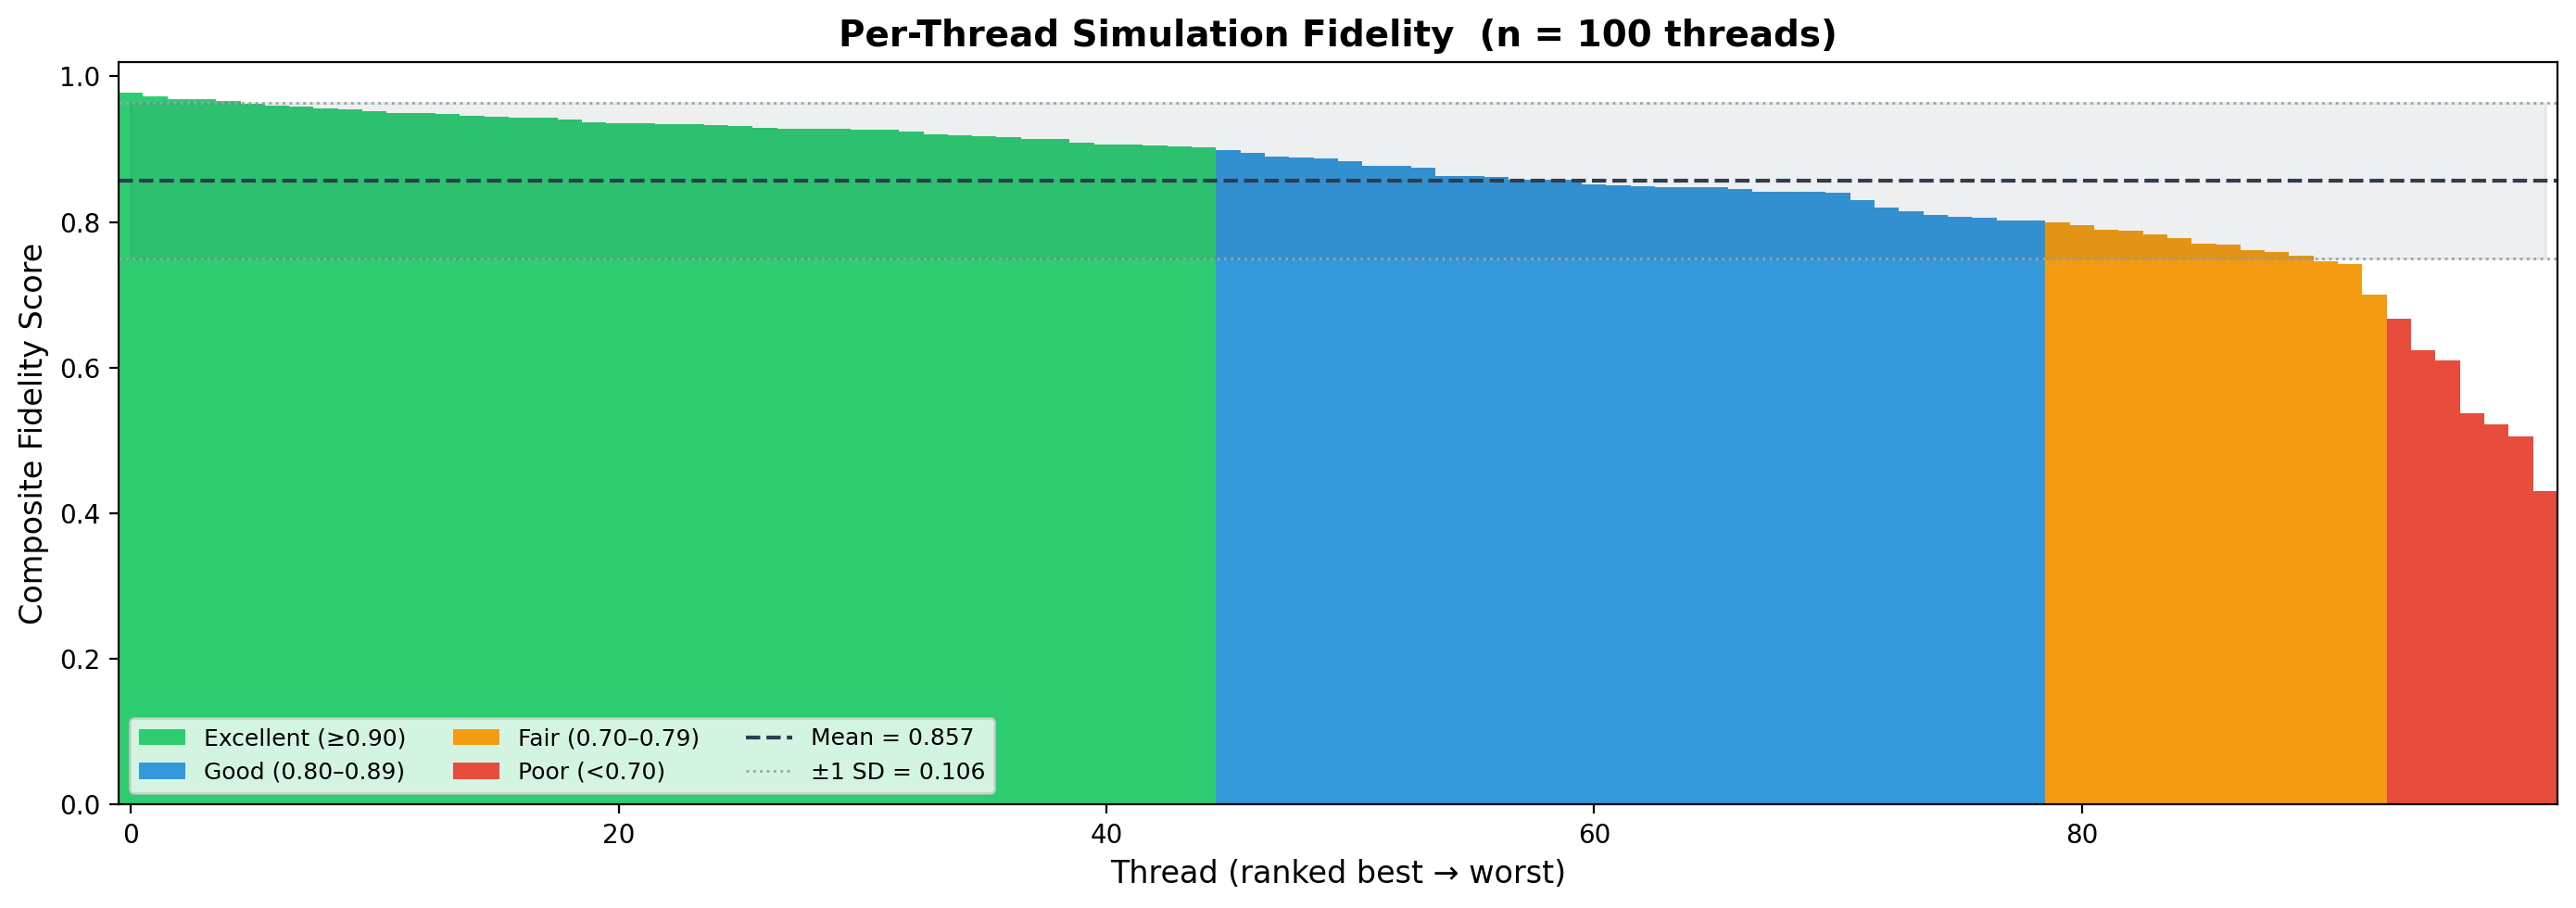
\includegraphics[width=\textwidth]{dissertation_figures/final/09_fidelity_scores_ranked.png}
\caption{All 100 threads ranked by composite fidelity score. Green: excellent ($\geq 0.90$); blue: good ($0.80$--$0.89$); amber: fair ($0.70$--$0.79$); red: poor ($< 0.70$). The dashed line indicates the mean; the shaded band indicates $\pm 1$ standard deviation.}
\label{fig:fidelity_ranked}
\end{figure}

% ------------------------------------------
\section{Parameter Sensitivity Analysis}
\label{sec:ablation_eval}

The ablation study evaluated 21 configurations across 10 threads each (210 total simulations). Each configuration was scored on a composite metric incorporating sentiment JSD, temporal decay, lexical diversity (TTR), semantic drift, emotion trajectory, Gini coefficient, Spearman rank correlation, and stance consistency. The full leaderboard is shown in Table~\ref{tab:ablation}.

\begin{table}[ht]
\centering
\caption{Top 10 ablation configurations ranked by composite score.}
\label{tab:ablation}
\begin{tabular}{clc}
\toprule
\textbf{Rank} & \textbf{Configuration} & \textbf{Composite Score} \\
\midrule
1 & 0-shot baseline                  & 0.780 \\
2 & Reply probability = 0.02        & 0.777 \\
3 & Old Rule 6 (hostile phrasing)    & 0.773 \\
4 & No dynamic scaling               & 0.755 \\
5 & Reply probability = 0.10         & 0.714 \\
6 & Context window = 15 posts        & 0.713 \\
7 & Temperature = 1.2                & 0.694 \\
8 & Old 4-tier aggression            & 0.677 \\
9 & Max tokens = 80                  & 0.634 \\
10 & Aggressive realist (multi-param) & 0.631 \\
\bottomrule
\end{tabular}
\end{table}

\subsection{Key Findings}

The top three configurations scored within 0.007 of each other (0.773--0.780), indicating that the optimised 0-shot baseline is near-optimal and stable under small perturbations. The most consequential parameter changes were:

\begin{enumerate}
\item \textbf{Vocabulary injection}: Removing vocabulary injection degraded performance substantially (rank 16, score 0.548), confirming that the politically charged keyword banks help anchor agent language to authentic partisan discourse.
\item \textbf{Temperature}: Higher temperature ($1.2$, score $0.694$) substantially outperformed lower temperature ($0.7$, score $0.451$). The increased randomness better captured the variability of real discourse.
\item \textbf{Context window}: Providing 15 posts of context ($0.713$) significantly outperformed 3 posts ($0.549$), confirming that agents require sufficient conversational context to calibrate their tone.
\item \textbf{Repetition penalty}: Increasing the repetition penalty from 1.1 to 1.3 degraded performance substantially ($0.429$), likely by disrupting the naturalness of generated text.
\item \textbf{Simulation length}: Extending from 10 to 20 rounds degraded performance ($0.411$), suggesting that longer simulations accumulate drift from the real distribution.
\end{enumerate}

Table~\ref{tab:ablation_deltas} provides a compact delta view relative to the 0-shot baseline for representative parameter changes.

\begin{table}[ht]
\centering
\caption{Ablation deltas relative to the 0-shot baseline (baseline: composite $=0.780$, sentiment JSD $=0.234$, temporal decay diff $=0.221$, stance consistency $=0.455$). Negative deltas are improvements for JSD/decay; positive deltas are improvements for composite/stance.}
\label{tab:ablation_deltas}
\small
\begin{tabular}{p{0.33\textwidth}rrrr}
\toprule
\textbf{Configuration} & $\Delta$ \textbf{Composite} & $\Delta$ \textbf{Sent. JSD} & $\Delta$ \textbf{Decay Diff} & $\Delta$ \textbf{Stance} \\
\midrule
Reply probability = 0.02 & -0.002 & -0.027 & +0.051 & +0.041 \\
Context window = 15       & -0.066 & +0.001 & +0.014 & +0.081 \\
Temperature = 1.2         & -0.085 & -0.012 & +0.050 & -0.031 \\
No vocabulary injection   & -0.231 & -0.002 & +0.044 & -0.029 \\
Repeat penalty = 1.3      & -0.351 & +0.021 & +0.019 & -0.032 \\
Rounds = 20               & -0.369 & +0.001 & +0.048 & -0.074 \\
\bottomrule
\end{tabular}
\end{table}

Figure~\ref{fig:heatmap} helps interpret these ablations at a glance. Rather than only showing final rank, it shows which configurations are consistently strong across sub-metrics and which succeed on one dimension while failing on others. The baseline and low-reply-probability settings are dark across most columns, which supports the claim that they are not narrowly overfitted to a single metric.

\begin{figure}[ht]
\centering
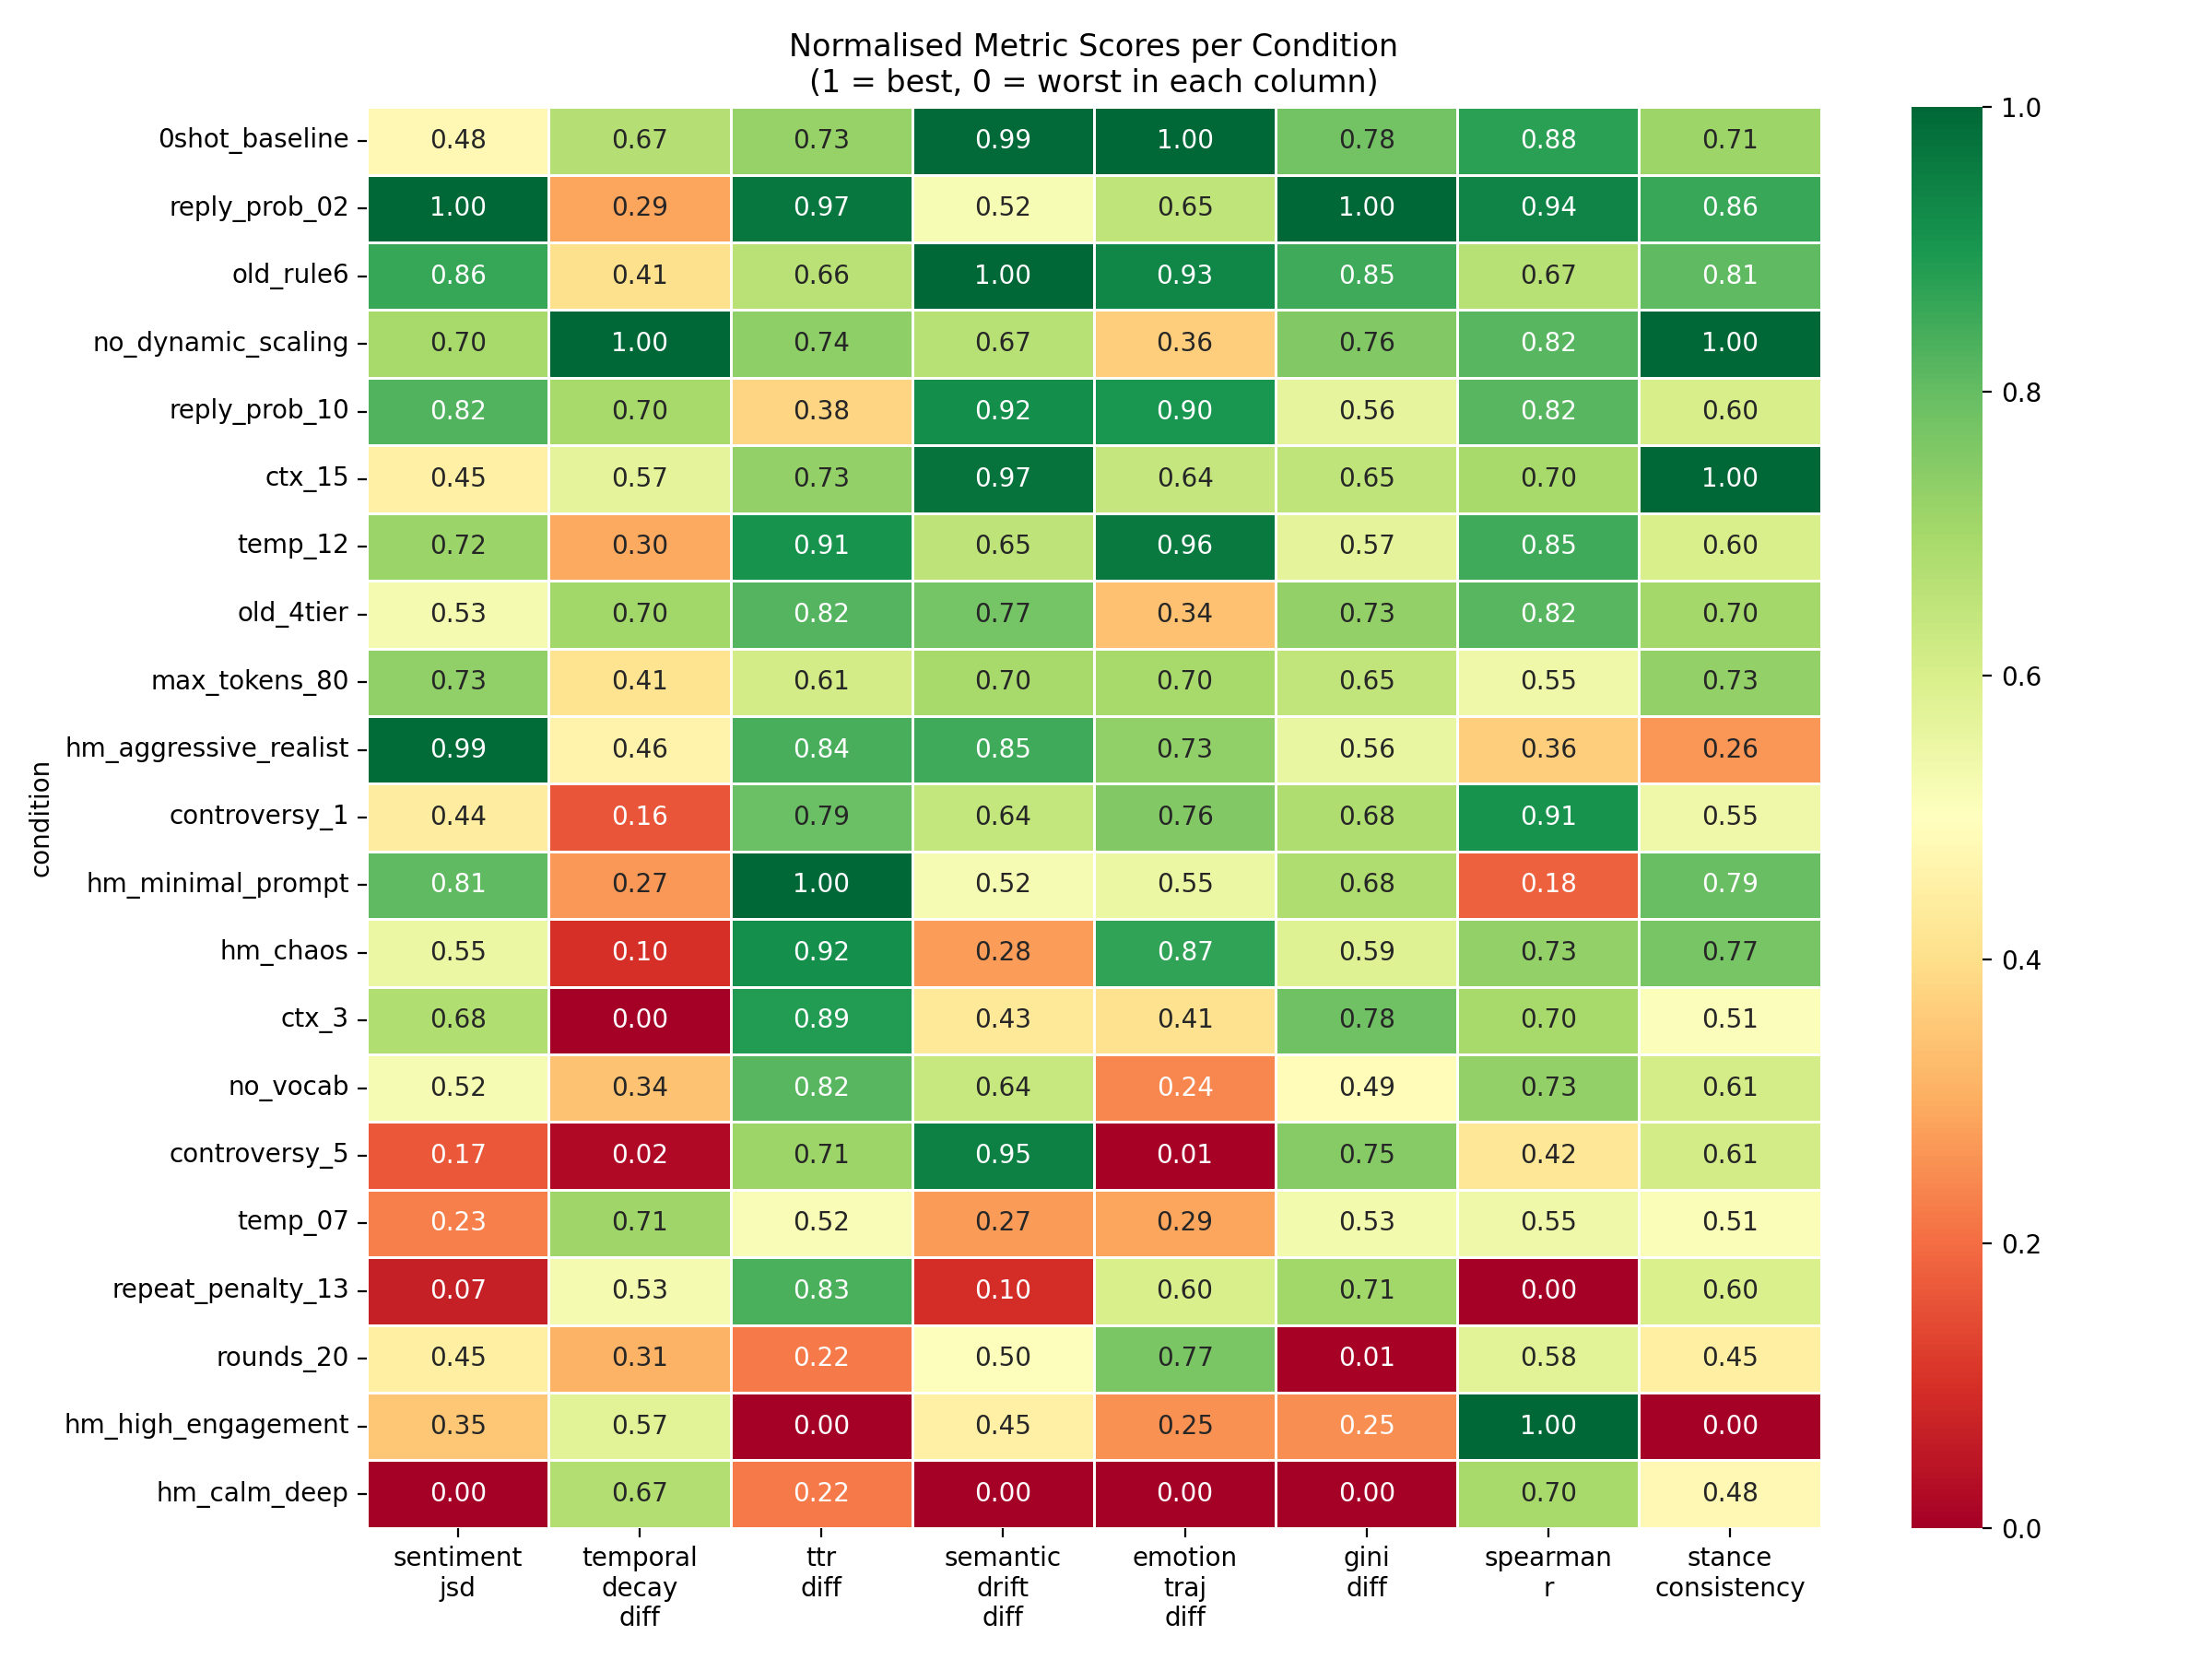
\includegraphics[width=\textwidth]{dissertation_figures/final/10_ablation_metric_heatmap.png}
\caption{Heatmap of normalised sub-metric scores across all 21 ablation configurations. Darker cells indicate better performance. The baseline and reply\_prob\_02 configurations show consistently strong performance across all metrics.}
\label{fig:heatmap}
\end{figure}

Figure~\ref{fig:leaderboard} makes the same point in ranked form. It shows that the best settings cluster closely together near the top, while a smaller set of parameter changes cause sharp performance collapse. That pattern is why the baseline is described as near-optimal but still diagnostically useful: there is limited headroom for improvement, yet clear room for degradation when key design choices are removed or mis-set.

\begin{figure}[ht]
\centering
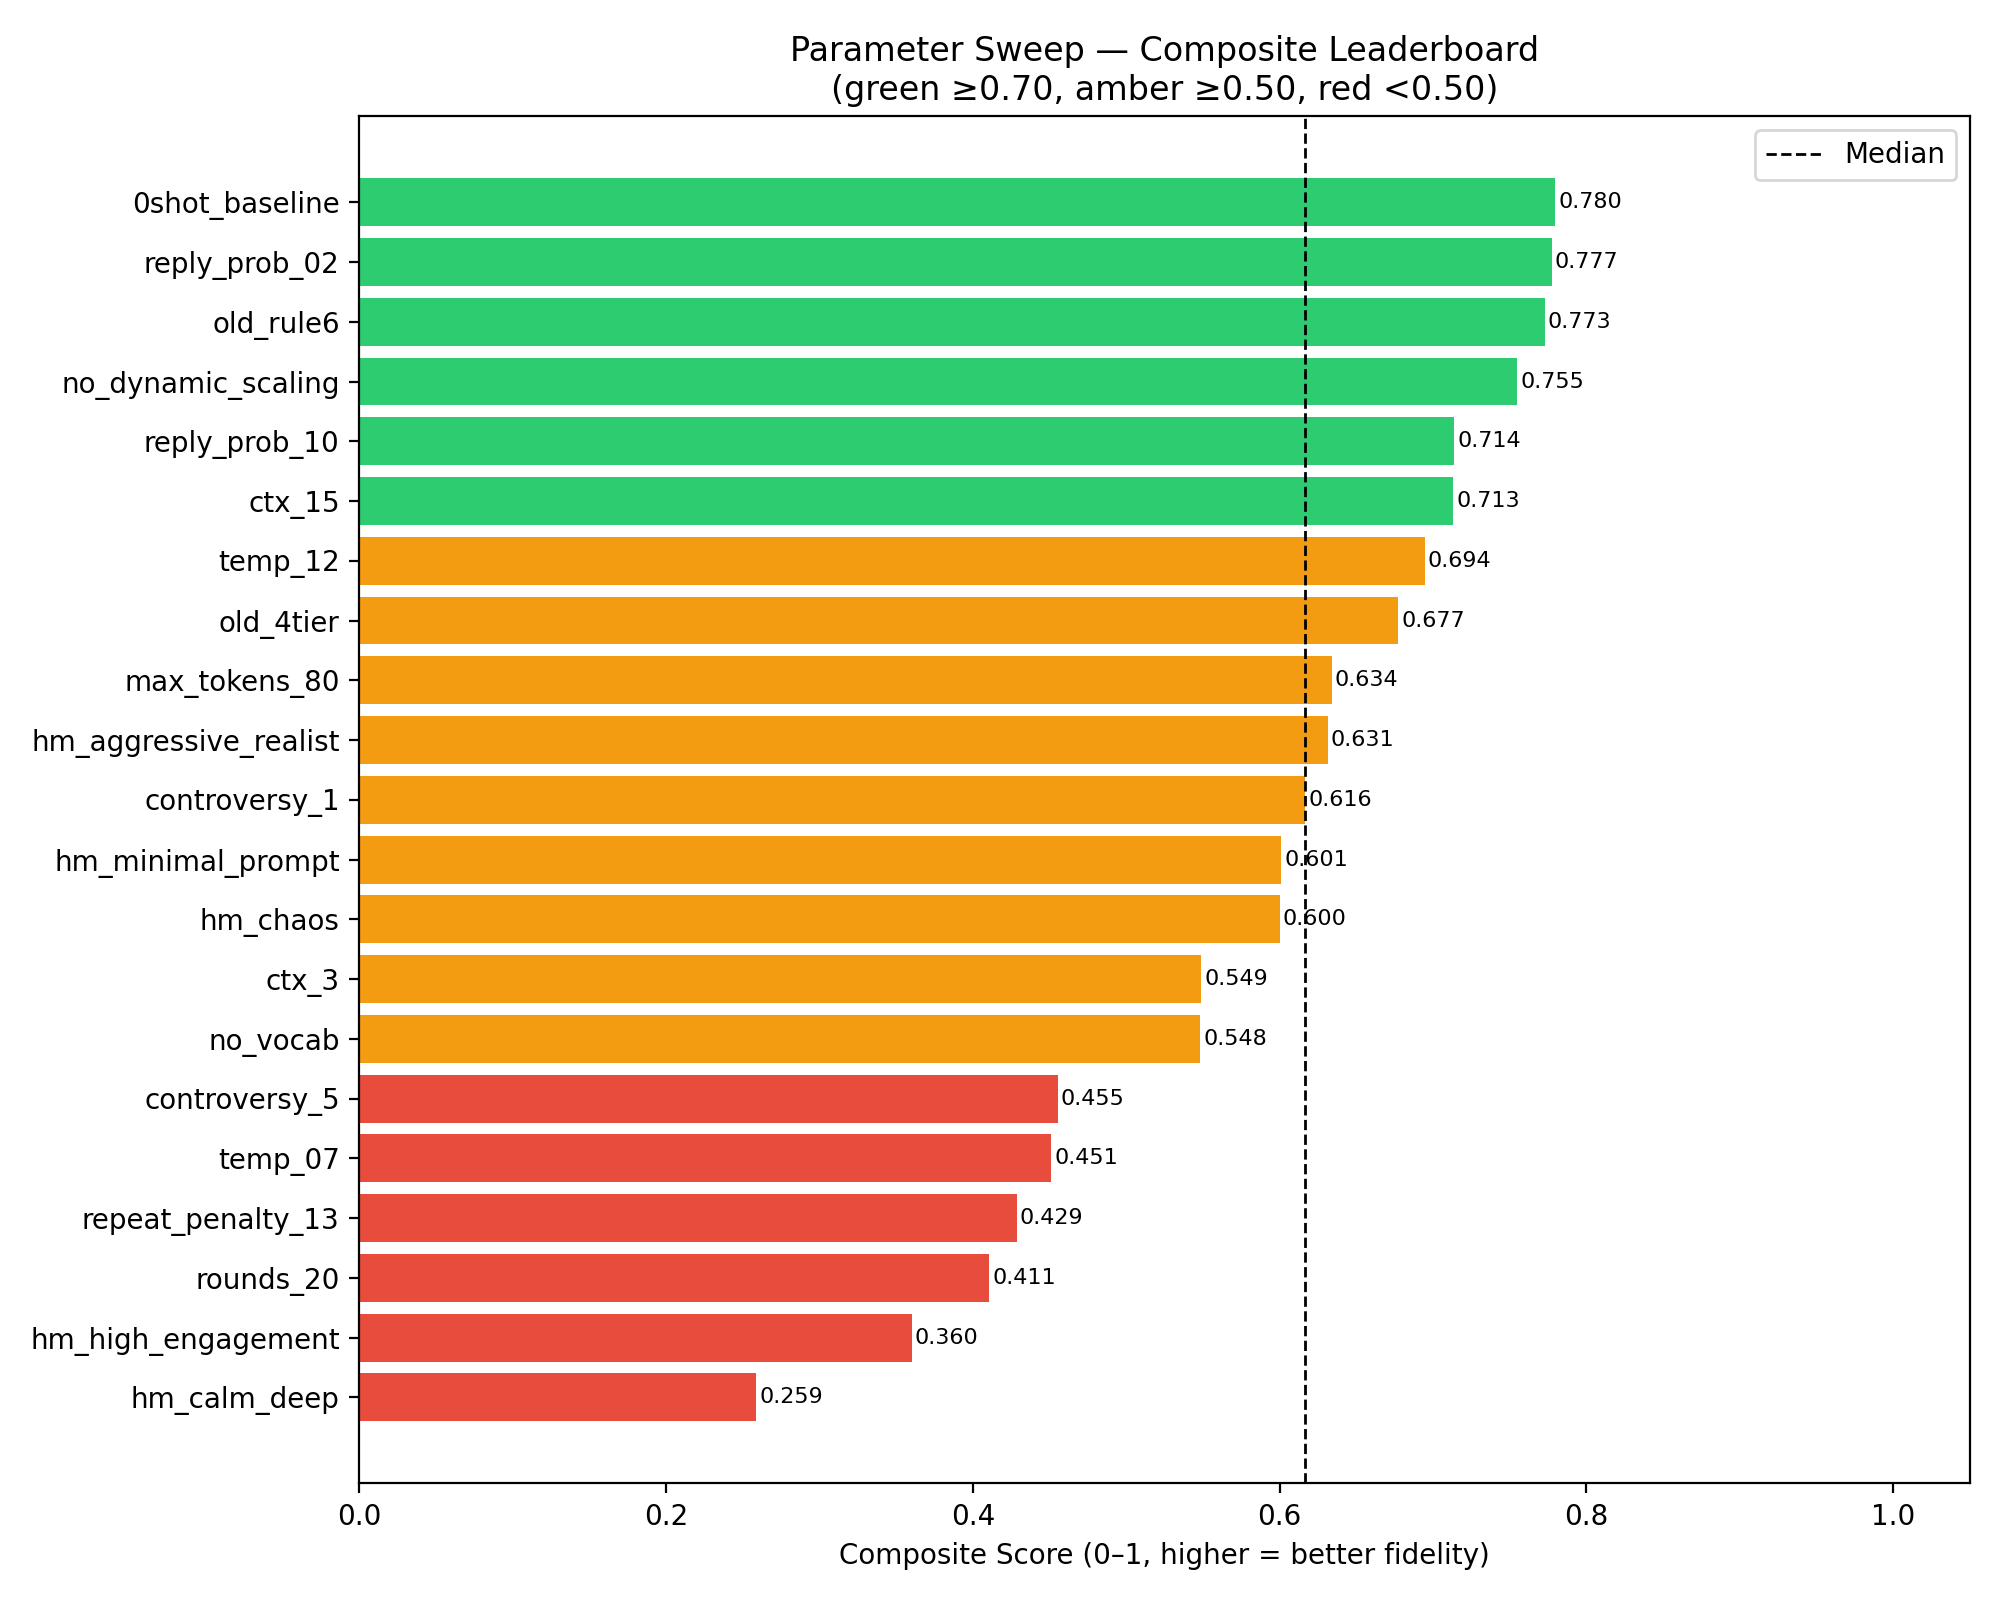
\includegraphics[width=0.85\textwidth]{dissertation_figures/final/11_ablation_leaderboard.png}
\caption{Composite scores for all 21 ablation configurations, ranked from best to worst.}
\label{fig:leaderboard}
\end{figure}

% ------------------------------------------
\section{Cross-Model Comparison}
\label{sec:crossmodel}

To test whether the simulation results are specific to the choice of language model, the full 100-thread evaluation was repeated with Qwen2.5~7B as the generation model, using identical agent populations, prompt templates, and parameter settings. Table~\ref{tab:crossmodel} compares the two models across all validation metrics.

\begin{table}[ht]
\centering
\caption{Cross-model comparison: Dolphin-Llama3 8B vs Qwen2.5 7B across 100 threads. Lower is better for all metrics except overall accuracy.}
\label{tab:crossmodel}
\begin{tabular}{lccc}
\toprule
\textbf{Metric} & \textbf{Llama} & \textbf{Qwen} & \textbf{Winner} \\
\midrule
Sentiment JSD         & \textbf{0.086} & 0.120 & Llama \\
Political JSD         & 0.039 & \textbf{0.013} & Qwen \\
Emotion JSD           & 0.118 & \textbf{0.092} & Qwen \\
Abs Sentiment Residual & \textbf{0.261} & 0.351 & Llama \\
Abs Aggression Gap    & \textbf{0.082} & 0.152 & Llama \\
Overall Accuracy (\%) & \textbf{92.3}  & 91.2  & Llama \\
\bottomrule
\end{tabular}
\end{table}

Dolphin-Llama3 8B achieves better sentiment calibration (JSD 0.086 vs 0.120), lower aggression gap (0.082 vs 0.152), and higher overall accuracy (92.3\% vs 91.2\%). Qwen2.5 7B produces more accurate political distributions (JSD 0.013 vs 0.039) and emotion distributions (JSD 0.092 vs 0.118). The table makes the trade-off clear without an extra figure: Qwen is stronger on political and emotion JSD, while Llama is clearly better on sentiment calibration, aggression calibration, and overall accuracy.

The most consequential difference is in sentiment bias. Llama exhibits no statistically significant sentiment bias (Wilcoxon $p = 0.633$), whereas Qwen exhibits a strong negative sentiment bias (Wilcoxon $p = 2.96 \times 10^{-17}$). This indicates that Qwen systematically generates more negative content than the real threads, a pattern similar to the pre-optimisation Llama results (Section~4.5.1). The cross-model comparison therefore confirms that model choice primarily affects sentiment and aggression calibration rather than political alignment, which remains comparatively stable across both models. The prompt engineering and agent construction methodology transfers across models, but sentiment calibration requires model-specific tuning.

% ------------------------------------------
\section{Discussion}
\label{sec:discussion}

\subsection{Summary of Results}

The central research question of this dissertation was whether a simulation pipeline can generate a realistic political reply thread from a root tweet and historically grounded agent profiles. Within the USC~X~24 setting, the answer is \emph{yes, to a useful but bounded degree}. Across 100 held-out threads, mean composite fidelity is $0.857 \pm 0.106$, with 79 threads scoring $\geq 0.80$ (Section~\ref{sec:fidelity}). Sentiment bias is not systematically directional (mean residual $+0.025$, Wilcoxon $p = 0.633$; Section~\ref{sec:100thread}), and political composition is the most accurately reproduced dimension (mean political JSD $= 0.039$). On the separate overall-accuracy metric, 97 of 100 threads are rated EXCELLENT. Read together, these results show that the pipeline is strong enough to support controlled downstream studies, while still leaving visible failure modes that bound the claim.

\subsection{Design and Parameter Justification}

For ABM systems, performance depends as much on behavioural assumptions as on model choice. The strongest design choices in this work are those supported by both mechanism and ablation evidence. First, synchronous activation reduces ordering artefacts by ensuring all agents respond to the same thread snapshot in each round. Second, aggression-calibrated prompting and dynamic scaling improve behavioural realism by making response tone depend on agent profile and thread context, rather than enforcing a fixed hostility prior. Third, conversational context length is critical: very short windows (3 posts) underperform substantially relative to longer windows, indicating that local discourse state is necessary for realistic generation. Fourth, higher generation temperature improved realism relative to conservative settings, suggesting that controlled stochasticity is required to match the heterogeneity of real political discourse. Finally, vocabulary injection was confirmed as beneficial by the ablation study: removing it degraded performance substantially, indicating that politically charged keyword banks help anchor agent language to authentic partisan discourse.

\subsection{Comparison with Prior Work}

Direct quantitative comparison with other LLM-based social simulation systems remains limited because studies use different targets, metrics, and datasets. The Italian election simulation~\citep{composta2025simulating} reports coalition-level interaction fidelity, whereas this dissertation evaluates thread-level distributional match across multiple dimensions. The two should therefore be read as complementary evidence for the broader feasibility of LLM-based social simulation rather than as benchmark-equivalent scores. Recent work on cross-partisan reply dynamics likewise shows that discourse outcomes depend strongly on audience composition and interaction context~\citep{cetinkaya2025crosspartisan}, which is consistent with the sensitivity patterns observed in the present ablation study.

Traditional opinion dynamics models~\citep{deffuant2000mixing,hegselmann2002opinion} provide mathematical frameworks for opinion evolution but do not produce text, making direct metric comparison impossible. The key advantage of the present LLM-based approach is that it generates natural language output that can be evaluated using the same automated tools applied to real social media data, enabling empirical validation that purely mathematical models cannot support~\citep{composta2025simulating,butler2024misinformation}.

\subsection{Research-Enabling Case Study: Re-testing Moral-Emotional Diffusion Claims}

This case study illustrates one of the most interesting uses of the pipeline: taking a claim from observational political-communication research and re-testing it under controlled counterfactual conditions. We do that in the setting of \citet{brady2017emotion}. Brady et al.\ analyse 563,312 tweets across climate change, gun control, and same-sex marriage (102,328; 47,373; and 413,611 respectively), using observational count models of retweet diffusion; in their corpus, 30\% of gun-control tweets, 23\% of same-sex-marriage tweets, and 29\% of climate tweets were retweeted at least once. Across those studies, moral-emotional language is associated with an average 20\% increase in retweet rate per additional moral-emotional word (mean IRR = 1.20), with topic-specific patterns such as positive moral-emotional effects for same-sex marriage (positive IRR = 1.92; negative IRR = 0.87) and negative-valence dominance for climate discourse (negative IRR = 1.31; positive IRR = 1.03, n.s.)~\citep{brady2017emotion}.

The key limitation of that design is that it compares \emph{different} tweets from \emph{different} users, audiences, and moments in time. The case-study protocol here removes most of that variation. For each topic (climate, gun, marriage), we use one base tweet, create three one-word variants plus a control, and run 12 simulated threads under fixed parameters, 10 rounds, and 0-shot generation. A single 100-agent population is reused across all conditions (40 Left, 40 Right, 20 Centre), with personas derived from the same five-model pipeline used elsewhere in the dissertation (political, emotion, sentiment, hate, offensive). The only manipulated variable is the lexical change in the root tweet.

Concrete examples from the run illustrate the design. Climate base tweet: ``Perciasepe: Global monitoring \& evaluation system for \#climatechange commitments is forming...'' with variants \emph{+loyal}, \emph{+vile}, and \emph{+good}. Gun base tweet: ``Do you \emph{hate} the fact that women hunt and kill deer...'' with variants \emph{+security}, \emph{hate $\rightarrow$ care}, and \emph{+brutal}. Marriage base tweet: ``...I know it's good luck, but the venue is outside'' with variants \emph{+goodness}, \emph{good $\rightarrow$ bad}, and \emph{+kill}.

Under those controlled conditions, one-word edits produced large downstream shifts, but not a simple universal ``positive word in, positive replies out'' pattern. Across the 9 edited conditions, the mean absolute net sentiment shift was 20.5 percentage points (median 18.1), and 6 of 9 edits moved net sentiment by more than 10 points relative to the control tweet. Reply volume was also sensitive: the mean absolute reply change was 9.9 posts (median 11), with 5 of 9 edits moving participation by at least 10 replies. In other words, the main result is not lexical valence consistency; it is that small wording changes can materially alter downstream thread behaviour under fixed audience composition.

That topic dependence is better understood as a strength of the instrument than as a failure of the case study. Real political discourse is context-sensitive and nonlinear: the same lexical change can cue reassurance, sarcasm, threat, or identity signalling differently across topics. A simulator that produced the same directional effect for every ``positive'' or ``negative'' word would arguably be less realistic. What matters here is that the pipeline is sensitive enough to detect substantial counterfactual differences while holding users, parameters, and interaction rules constant.

Concrete examples still illustrate the range of effects. Climate \emph{+loyal} shifted net sentiment by +34.6 points; climate \emph{+vile} shifted it by -14.0 points. In the gun topic, \emph{hate $\rightarrow$ care} shifted net sentiment by +18.1 points. In the marriage topic, \emph{+kill} shifted net sentiment by -52.4 points, while \emph{+goodness} increased reply volume by +29. These are not trivial fluctuations: they are large enough to show that the pipeline can be used to probe which specific message edits materially change simulated discourse outcomes.

This comparison shows where the pipeline changes the methodological question. Brady et al.\ establish observational diffusion regularities at scale; the present system adds controlled, within-message counterfactual testing. Instead of only asking which language features correlate with spread in heterogeneous real-world data, we can ask what changes when one word is edited while audience composition and behavioural assumptions are held constant. That same design pattern is useful beyond this example: it can support research replications, communication experiments, and bounded product-side message testing, provided the target population remains close to the evaluated setting.

\subsection{Failure Modes}

The dominant failure mode is sentiment polarity inversion. In 7 of 100 threads (fidelity $< 0.70$), generated sentiment moves in the opposite direction to the real thread. These cases appear to arise when the root tweet alone is an insufficient predictor of downstream tone (e.g., rallying, ironic, or humour-driven replies). A second weakness is partial hostility miscalibration: although aggression tracks real threads in the correct direction, the effect size is moderate ($r = 0.332$), indicating that tone intensity is captured only coarsely. Taken together, these errors indicate that the model is strongest on macro-distributional realism and weaker on fine-grained affective trajectory prediction.

\subsection{Limitations}

The limitations can be interpreted as four threats to validity. \textit{Construct validity}: all outcomes are measured through automated classifiers, so any systematic classifier bias directly affects both error estimates and apparent agreement. \textit{Internal validity}: several behavioural mechanisms (bounded confidence threshold, aggression scaling, round limit) are hand-specified and tuned, so alternative yet plausible formulations could yield different outcomes. \textit{External validity}: evaluation uses one dataset (USC~X~24) from one platform and one election context, so transfer to other political systems, languages, or platform affordances remains unverified. \textit{Analytical validity}: composite fidelity depends on chosen metric weights and normalisation caps; different weighting schemes may change model rankings even when raw sub-metrics are unchanged. These constraints do not invalidate the present findings, but they bound the claims: this work provides strong evidence of feasibility in a defined setting rather than a universal model of online reaction dynamics.

A further boundary condition is persona conditioning. Agent behaviour is conditioned on historically aggregated user profiles derived from prior tweets, and the strongest results should therefore be interpreted as \emph{conditional fidelity under history-informed agent profiles}. This supports a meaningful forward-simulation claim in the USC~X~24 setting, but not a claim that the model captures general human behaviour independently of persona information. Establishing that stronger claim requires explicit counterfactual baselines (e.g., demographic-matched random agents and no-persona agents) evaluated under identical protocols.

% ==========================================
% CHAPTER 6: CONCLUSIONS
% ==========================================
\chapter{Conclusions}

\section{Conclusion}
This dissertation asked whether a forward-looking simulation pipeline can generate realistic political reply threads from only a root tweet and historically grounded agent profiles. The results show that it can, to a useful but bounded degree. Across 100 held-out threads, the optimised Dolphin-Llama3~8B pipeline achieved mean JSD values of 0.086 (sentiment), 0.039 (political), and 0.118 (emotion), with mean overall accuracy of $92.3\% \pm 4.6\%$ and composite fidelity of $0.857 \pm 0.106$. Sentiment bias was not statistically directional (mean residual $+0.025$, Wilcoxon $p = 0.633$), indicating that the final system no longer exhibits the strong negative drift observed in the initial configuration.

Methodologically, the main contribution is a new research instrument: an end-to-end ABM+LLM pipeline that can run forward and counterfactual thread-level experiments, rather than only retrospective engagement analyses. The case study shows why that matters. Once the pipeline is validated, it can be used to revisit claims from observational work under fixed audience composition and controlled lexical changes. The same capability is also relevant to bounded pre-deployment message testing, where the question is not ``will this go viral?'' but ``how might discourse shift if the wording changes?''

The contribution is not a universal model of online political behaviour. It is a validated simulation framework with clear operational boundaries, supported by multi-metric evaluation, ablation evidence, and cross-model comparison, that enables previously hard-to-test questions about downstream discourse effects. The ablation and model-comparison results are especially informative for future systems design: performance proved sensitive to context length, generation temperature, reply probability, and vocabulary conditioning, while cross-model transfer showed that sentiment and aggression calibration are model-dependent whereas political-distribution alignment is comparatively stable. These findings turn implementation choices into testable design guidance rather than ad hoc prompt heuristics.

\section{Future Directions}
Future work should focus on robustness, causal attribution, and external validity:
\begin{enumerate}
\item \textbf{Persona-dependence ablations}: run matched baselines with demographic-random and no-persona agents to quantify how much fidelity is attributable to history-informed personas.
\item \textbf{Broader domains}: evaluate on non-election periods, non-US political contexts, and multilingual datasets to test external validity.
\item \textbf{Temporal and structural realism}: extend the simulator with event-time modelling and platform-specific interaction constraints, then validate against reconstructed reply-chain dynamics where available.
\item \textbf{Classifier uncertainty}: propagate confidence intervals from the five RoBERTa classifiers into downstream metrics so reported fidelity includes measurement uncertainty.
\item \textbf{Human evaluation}: supplement automated metrics with blinded human judgements of realism, stance plausibility, and conversational coherence.
\end{enumerate}

\bibliographystyle{unsrtnat}
\bibliography{mybibfile}

\appendix
\chapter{Reproducibility Notes}
All reported evaluation results are produced from fixed batch outputs and scripts in the project repository. Core artefacts are stored under \texttt{analysis/} (metrics and summary tables), \texttt{outputs/} (thread-level simulation outputs), and \texttt{dissertation\_figures/} (final figure assets referenced in this document). The 100-thread validation, ablation study, and cross-model comparison were each executed with explicit run manifests and per-thread logs to support auditability and rerun verification.

\end{document}
